\documentclass{standalone}
\begin{document}
\begin{table}[!htb]
	\centering
	\caption{Figure \ref{fig:graph_1001} Configuration File}
	\label{tab:graph_1001}
	\begin{tabular}{| c | c |}
		\hline
		Mutation Algorithm		& Move		 \\
		\hline
		Fitness Evaluations		& 10000		 \\
		\hline
		Tournament Size For Survival Selection		& 5		 \\
		\hline
		Mutation Rate		& 0.1		 \\
		\hline
		Self Adaptive Penalty Coefficient		& False		 \\
		\hline
		Random Seed		& 1001		 \\
		\hline
		Population Size		& 100		 \\
		\hline
		Placement Algorithm		& Random		 \\
		\hline
		Termination Convergence Criterion		& 10000		 \\
		\hline
		Survival Strategy		& Plus		 \\
		\hline
		Runs		& 30		 \\
		\hline
		Survivor Algorithm		& Truncation		 \\
		\hline
		Offspring Count		& 50		 \\
		\hline
		Solution File Path		& None		 \\
		\hline
		Self Adaptive Mutation Rate		& False		 \\
		\hline
		Search Algorithm		& EA		 \\
		\hline
		Parent Selection Algorithm		& k-Tournament Selection with replacement		 \\
		\hline
		Self Adaptive Offspring Count		& False		 \\
		\hline
		Log File Path		& None		 \\
		\hline
		MOEA		& True		 \\
		\hline
		Recombination Algorithm		& Partially Mapped Crossover		 \\
		\hline
		Tournament Size For Parent Selection		& 5		 \\
		\hline
		Penalty Coefficient		& 1		 \\
		\hline
	\end{tabular}
\end{table}
\begin{figure}[!htb]
	\caption{Input 1}
	\label{fig:graph_1001}
	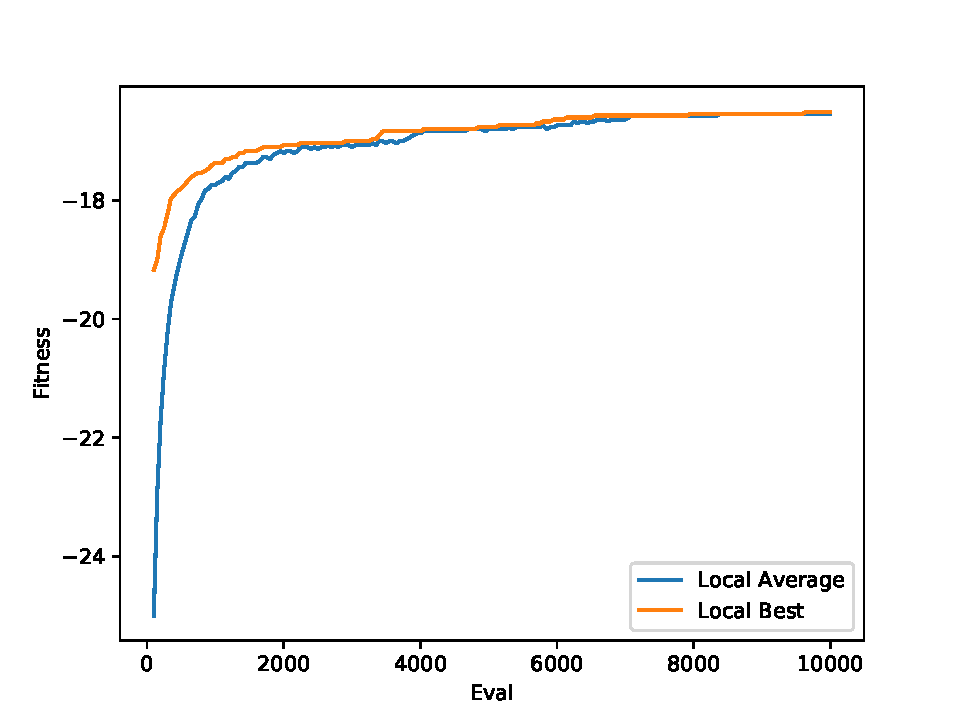
\includegraphics[width=\textwidth]{../graphs/graphs/1001.pdf}
\end{figure}


\begin{figure}[!htb]
	\caption{Figure \ref{fig:graph_1001} Representation}
	\label{fig:picture_1001}
	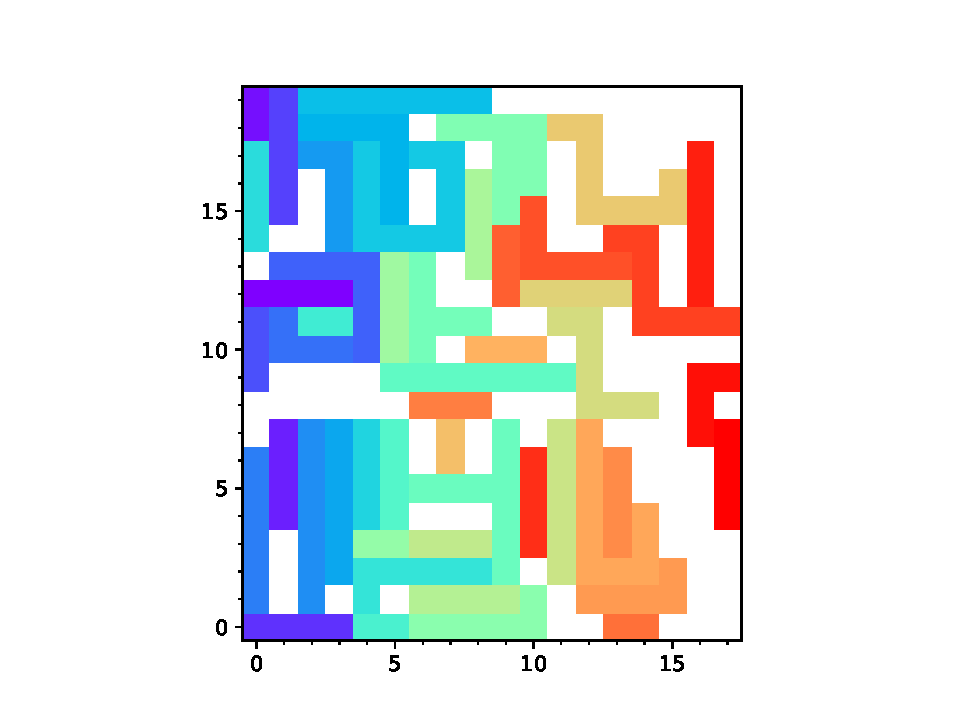
\includegraphics[width=\textwidth]{../graphs/picture/1001.pdf}
\end{figure}


\begin{table}[!htb]
	\centering
	\caption{Figure \ref{fig:graph_1002} Configuration File}
	\label{tab:graph_1002}
	\begin{tabular}{| c | c |}
		\hline
		Mutation Algorithm		& Flip		 \\
		\hline
		Fitness Evaluations		& 10000		 \\
		\hline
		Tournament Size For Survival Selection		& 5		 \\
		\hline
		Mutation Rate		& 0.1		 \\
		\hline
		Self Adaptive Penalty Coefficient		& False		 \\
		\hline
		Random Seed		& 1002		 \\
		\hline
		Population Size		& 100		 \\
		\hline
		Placement Algorithm		& Random		 \\
		\hline
		Termination Convergence Criterion		& 10000		 \\
		\hline
		Survival Strategy		& Plus		 \\
		\hline
		Runs		& 30		 \\
		\hline
		Survivor Algorithm		& Truncation		 \\
		\hline
		Offspring Count		& 50		 \\
		\hline
		Solution File Path		& None		 \\
		\hline
		Self Adaptive Mutation Rate		& False		 \\
		\hline
		Search Algorithm		& EA		 \\
		\hline
		Parent Selection Algorithm		& k-Tournament Selection with replacement		 \\
		\hline
		Self Adaptive Offspring Count		& False		 \\
		\hline
		Log File Path		& None		 \\
		\hline
		MOEA		& True		 \\
		\hline
		Recombination Algorithm		& Partially Mapped Crossover		 \\
		\hline
		Tournament Size For Parent Selection		& 5		 \\
		\hline
		Penalty Coefficient		& 1		 \\
		\hline
	\end{tabular}
\end{table}
\begin{figure}[!htb]
	\caption{Input 1}
	\label{fig:graph_1002}
	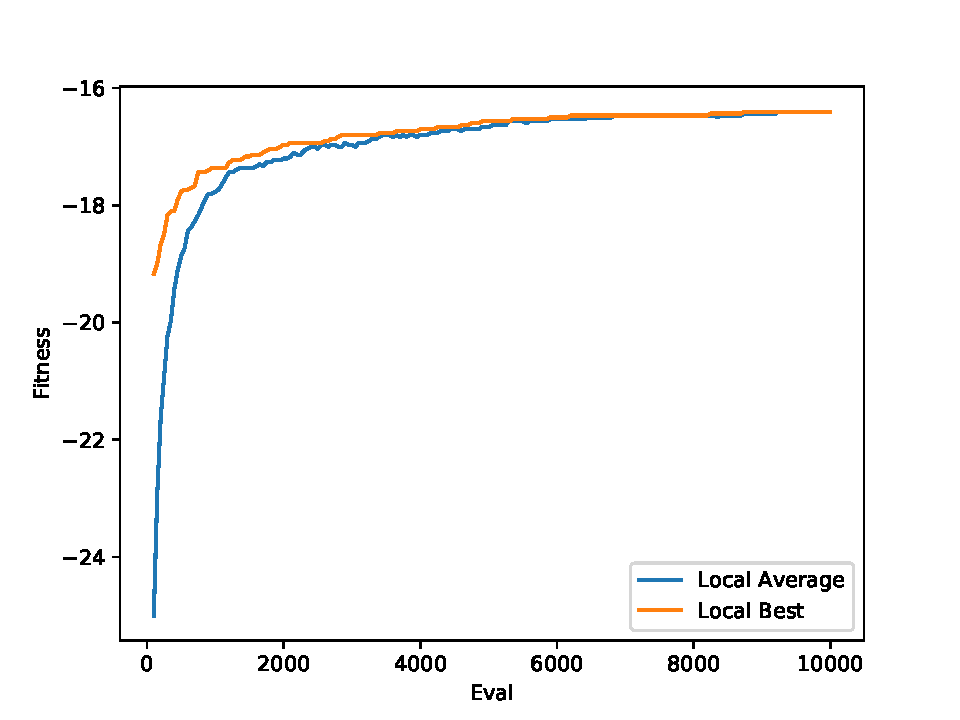
\includegraphics[width=\textwidth]{../graphs/graphs/1002.pdf}
\end{figure}


\begin{figure}[!htb]
	\caption{Figure \ref{fig:graph_1002} Representation}
	\label{fig:picture_1002}
	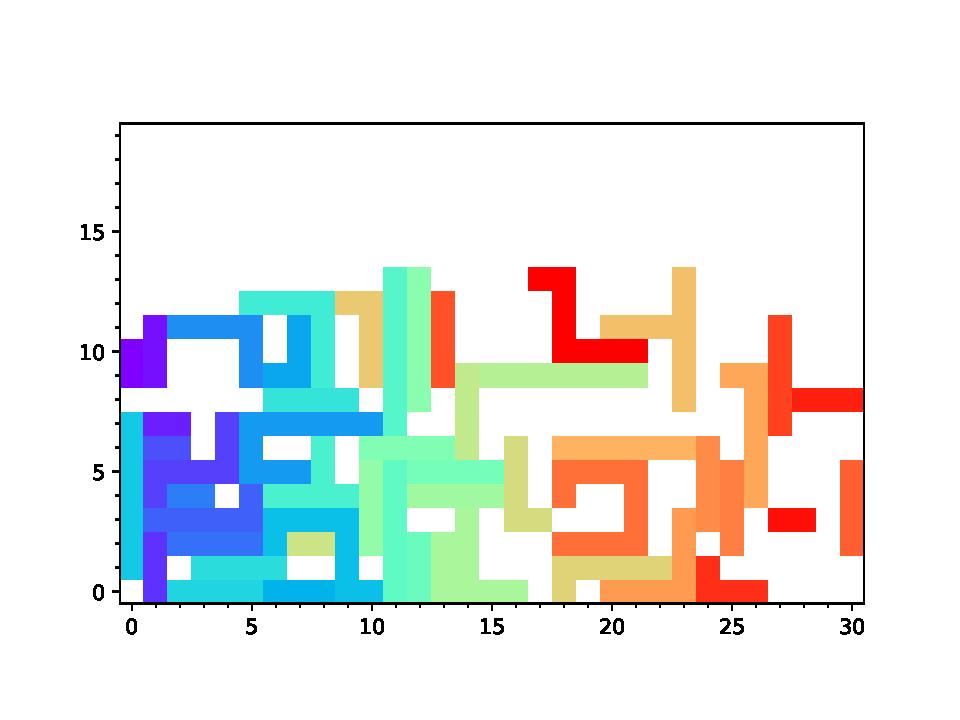
\includegraphics[width=\textwidth]{../graphs/picture/1002.pdf}
\end{figure}


\begin{table}[!htb]
	\centering
	\caption{Figure \ref{fig:graph_1003} Configuration File}
	\label{tab:graph_1003}
	\begin{tabular}{| c | c |}
		\hline
		Mutation Algorithm		& Move		 \\
		\hline
		Fitness Evaluations		& 10000		 \\
		\hline
		Tournament Size For Survival Selection		& 5		 \\
		\hline
		Mutation Rate		& 0.1		 \\
		\hline
		Self Adaptive Penalty Coefficient		& False		 \\
		\hline
		Random Seed		& 1003		 \\
		\hline
		Population Size		& 100		 \\
		\hline
		Placement Algorithm		& Random		 \\
		\hline
		Termination Convergence Criterion		& 10000		 \\
		\hline
		Survival Strategy		& Plus		 \\
		\hline
		Runs		& 30		 \\
		\hline
		Survivor Algorithm		& Truncation		 \\
		\hline
		Offspring Count		& 50		 \\
		\hline
		Solution File Path		& None		 \\
		\hline
		Self Adaptive Mutation Rate		& False		 \\
		\hline
		Search Algorithm		& EA		 \\
		\hline
		Parent Selection Algorithm		& Fitness Proportional Selection		 \\
		\hline
		Self Adaptive Offspring Count		& False		 \\
		\hline
		Log File Path		& None		 \\
		\hline
		MOEA		& True		 \\
		\hline
		Recombination Algorithm		& Partially Mapped Crossover		 \\
		\hline
		Tournament Size For Parent Selection		& 5		 \\
		\hline
		Penalty Coefficient		& 1		 \\
		\hline
	\end{tabular}
\end{table}
\begin{figure}[!htb]
	\caption{Input 1}
	\label{fig:graph_1003}
	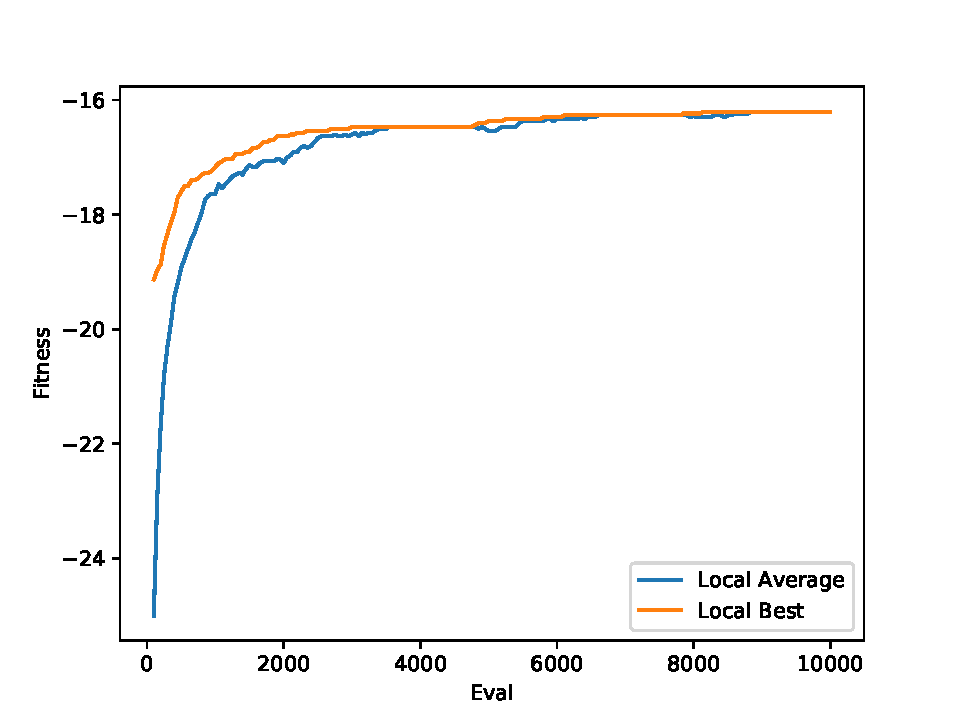
\includegraphics[width=\textwidth]{../graphs/graphs/1003.pdf}
\end{figure}


\begin{figure}[!htb]
	\caption{Figure \ref{fig:graph_1003} Representation}
	\label{fig:picture_1003}
	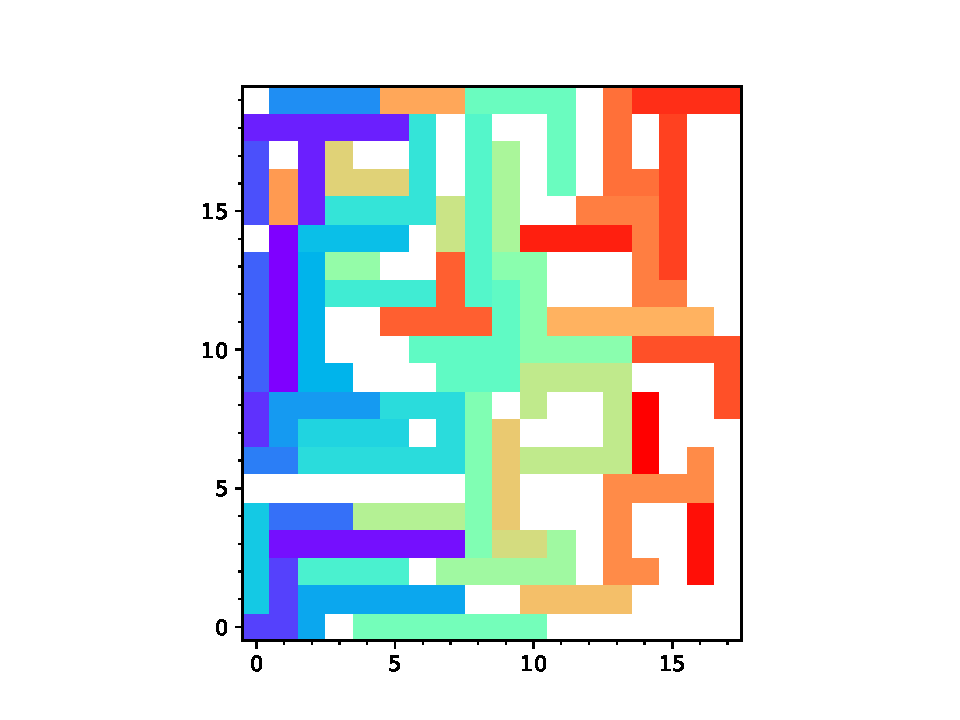
\includegraphics[width=\textwidth]{../graphs/picture/1003.pdf}
\end{figure}


\begin{table}[!htb]
	\centering
	\caption{Figure \ref{fig:graph_1004} Configuration File}
	\label{tab:graph_1004}
	\begin{tabular}{| c | c |}
		\hline
		Mutation Algorithm		& Flip		 \\
		\hline
		Fitness Evaluations		& 10000		 \\
		\hline
		Tournament Size For Survival Selection		& 5		 \\
		\hline
		Mutation Rate		& 0.1		 \\
		\hline
		Self Adaptive Penalty Coefficient		& False		 \\
		\hline
		Random Seed		& 1004		 \\
		\hline
		Population Size		& 100		 \\
		\hline
		Placement Algorithm		& Random		 \\
		\hline
		Termination Convergence Criterion		& 10000		 \\
		\hline
		Survival Strategy		& Plus		 \\
		\hline
		Runs		& 30		 \\
		\hline
		Survivor Algorithm		& Truncation		 \\
		\hline
		Offspring Count		& 50		 \\
		\hline
		Solution File Path		& None		 \\
		\hline
		Self Adaptive Mutation Rate		& False		 \\
		\hline
		Search Algorithm		& EA		 \\
		\hline
		Parent Selection Algorithm		& Fitness Proportional Selection		 \\
		\hline
		Self Adaptive Offspring Count		& False		 \\
		\hline
		Log File Path		& None		 \\
		\hline
		MOEA		& True		 \\
		\hline
		Recombination Algorithm		& Partially Mapped Crossover		 \\
		\hline
		Tournament Size For Parent Selection		& 5		 \\
		\hline
		Penalty Coefficient		& 1		 \\
		\hline
	\end{tabular}
\end{table}
\begin{figure}[!htb]
	\caption{Input 1}
	\label{fig:graph_1004}
	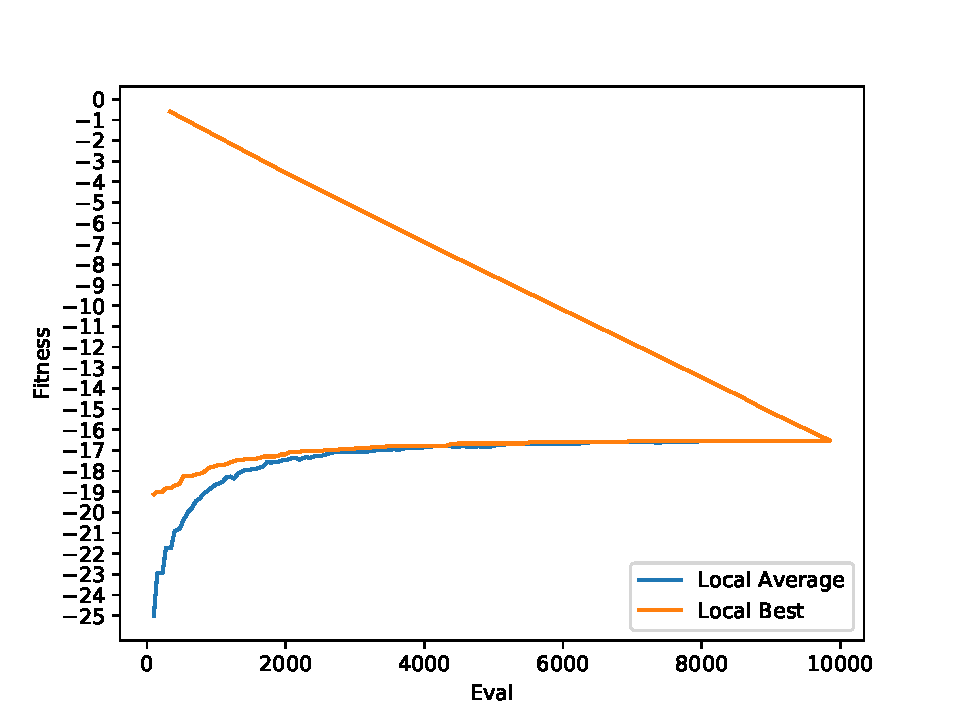
\includegraphics[width=\textwidth]{../graphs/graphs/1004.pdf}
\end{figure}


\begin{figure}[!htb]
	\caption{Figure \ref{fig:graph_1004} Representation}
	\label{fig:picture_1004}
	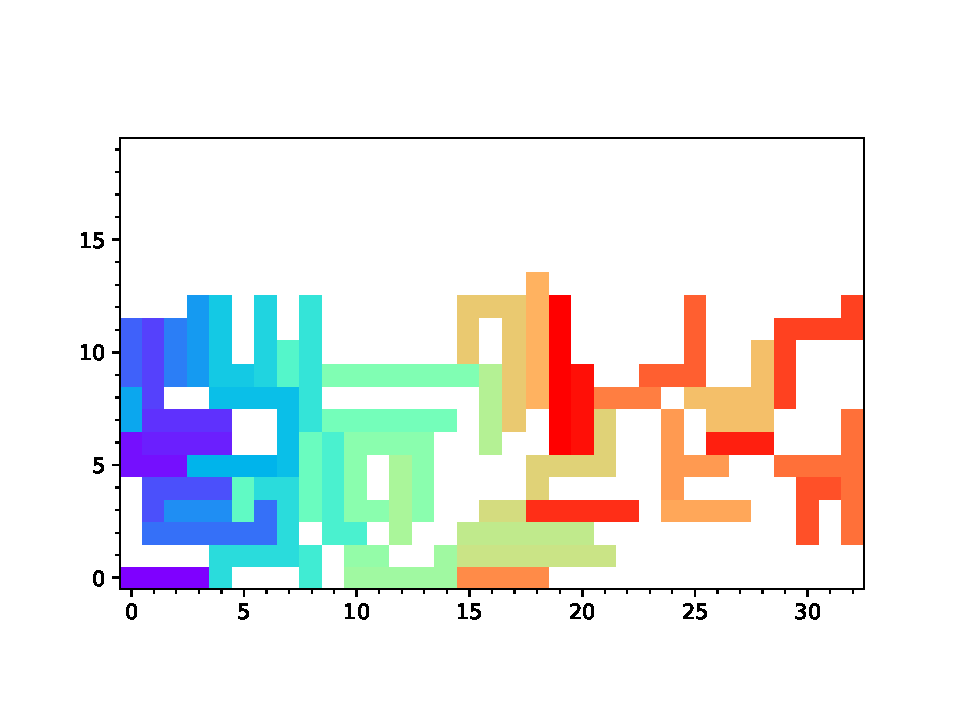
\includegraphics[width=\textwidth]{../graphs/picture/1004.pdf}
\end{figure}


\begin{table}[!htb]
	\centering
	\caption{Figure \ref{fig:graph_1005} Configuration File}
	\label{tab:graph_1005}
	\begin{tabular}{| c | c |}
		\hline
		Mutation Algorithm		& Move		 \\
		\hline
		Fitness Evaluations		& 10000		 \\
		\hline
		Tournament Size For Survival Selection		& 5		 \\
		\hline
		Mutation Rate		& 0.1		 \\
		\hline
		Self Adaptive Penalty Coefficient		& False		 \\
		\hline
		Random Seed		& 1005		 \\
		\hline
		Population Size		& 100		 \\
		\hline
		Placement Algorithm		& Random		 \\
		\hline
		Termination Convergence Criterion		& 10000		 \\
		\hline
		Survival Strategy		& Plus		 \\
		\hline
		Runs		& 30		 \\
		\hline
		Survivor Algorithm		& Truncation		 \\
		\hline
		Offspring Count		& 50		 \\
		\hline
		Solution File Path		& None		 \\
		\hline
		Self Adaptive Mutation Rate		& False		 \\
		\hline
		Search Algorithm		& EA		 \\
		\hline
		Parent Selection Algorithm		& Uniform Random		 \\
		\hline
		Self Adaptive Offspring Count		& False		 \\
		\hline
		Log File Path		& None		 \\
		\hline
		MOEA		& True		 \\
		\hline
		Recombination Algorithm		& Partially Mapped Crossover		 \\
		\hline
		Tournament Size For Parent Selection		& 5		 \\
		\hline
		Penalty Coefficient		& 1		 \\
		\hline
	\end{tabular}
\end{table}
\begin{figure}[!htb]
	\caption{Input 1}
	\label{fig:graph_1005}
	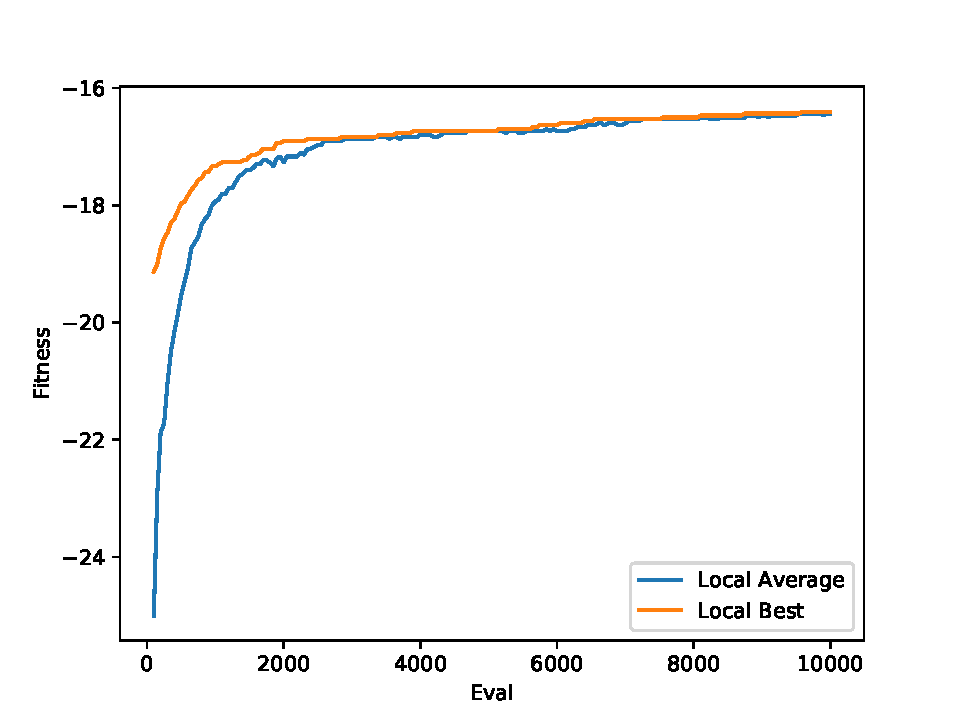
\includegraphics[width=\textwidth]{../graphs/graphs/1005.pdf}
\end{figure}


\begin{figure}[!htb]
	\caption{Figure \ref{fig:graph_1005} Representation}
	\label{fig:picture_1005}
	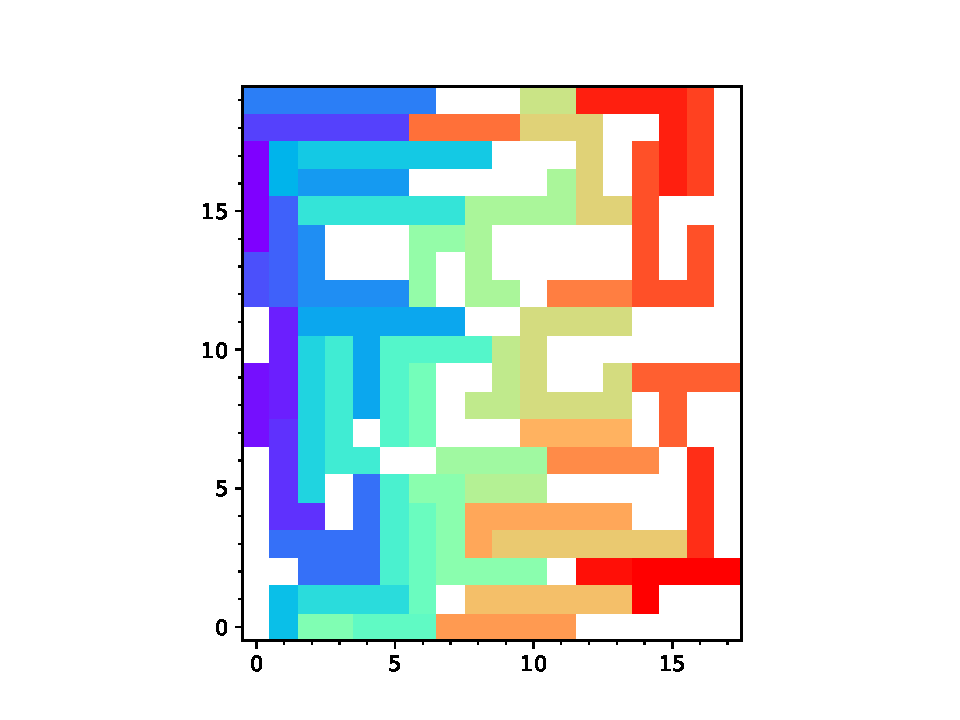
\includegraphics[width=\textwidth]{../graphs/picture/1005.pdf}
\end{figure}


\begin{table}[!htb]
	\centering
	\caption{Figure \ref{fig:graph_1006} Configuration File}
	\label{tab:graph_1006}
	\begin{tabular}{| c | c |}
		\hline
		Mutation Algorithm		& Flip		 \\
		\hline
		Fitness Evaluations		& 10000		 \\
		\hline
		Tournament Size For Survival Selection		& 5		 \\
		\hline
		Mutation Rate		& 0.1		 \\
		\hline
		Self Adaptive Penalty Coefficient		& False		 \\
		\hline
		Random Seed		& 1006		 \\
		\hline
		Population Size		& 100		 \\
		\hline
		Placement Algorithm		& Random		 \\
		\hline
		Termination Convergence Criterion		& 10000		 \\
		\hline
		Survival Strategy		& Plus		 \\
		\hline
		Runs		& 30		 \\
		\hline
		Survivor Algorithm		& Truncation		 \\
		\hline
		Offspring Count		& 50		 \\
		\hline
		Solution File Path		& None		 \\
		\hline
		Self Adaptive Mutation Rate		& False		 \\
		\hline
		Search Algorithm		& EA		 \\
		\hline
		Parent Selection Algorithm		& Uniform Random		 \\
		\hline
		Self Adaptive Offspring Count		& False		 \\
		\hline
		Log File Path		& None		 \\
		\hline
		MOEA		& True		 \\
		\hline
		Recombination Algorithm		& Partially Mapped Crossover		 \\
		\hline
		Tournament Size For Parent Selection		& 5		 \\
		\hline
		Penalty Coefficient		& 1		 \\
		\hline
	\end{tabular}
\end{table}
\begin{figure}[!htb]
	\caption{Input 1}
	\label{fig:graph_1006}
	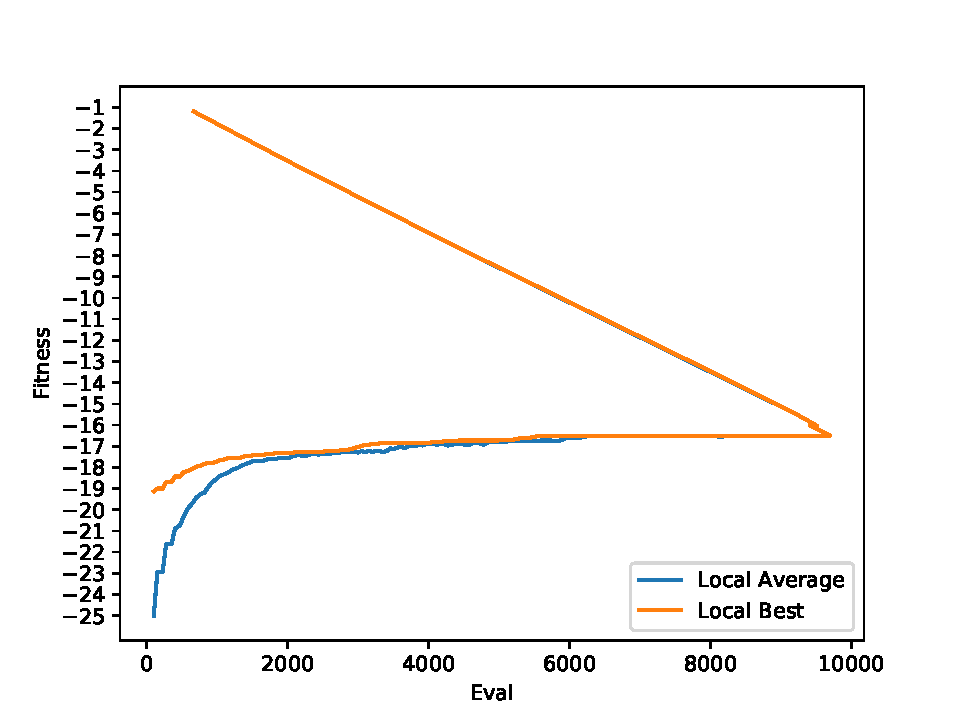
\includegraphics[width=\textwidth]{../graphs/graphs/1006.pdf}
\end{figure}


\begin{figure}[!htb]
	\caption{Figure \ref{fig:graph_1006} Representation}
	\label{fig:picture_1006}
	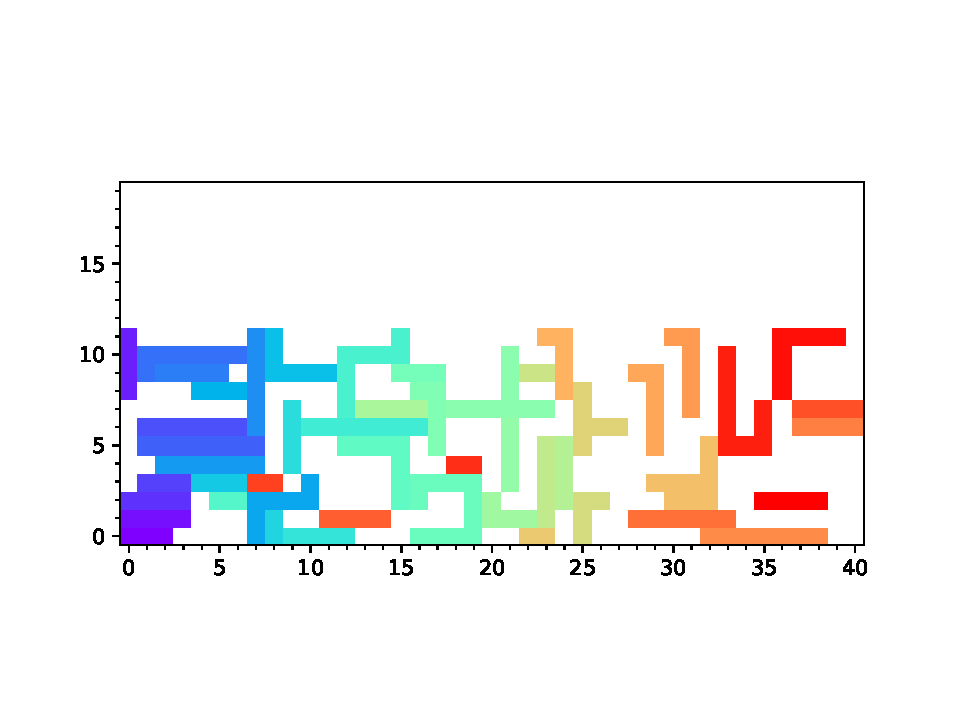
\includegraphics[width=\textwidth]{../graphs/picture/1006.pdf}
\end{figure}


\begin{table}[!htb]
	\centering
	\caption{Figure \ref{fig:graph_1007} Configuration File}
	\label{tab:graph_1007}
	\begin{tabular}{| c | c |}
		\hline
		Mutation Algorithm		& Move		 \\
		\hline
		Fitness Evaluations		& 10000		 \\
		\hline
		Tournament Size For Survival Selection		& 5		 \\
		\hline
		Mutation Rate		& 0.1		 \\
		\hline
		Self Adaptive Penalty Coefficient		& False		 \\
		\hline
		Random Seed		& 1007		 \\
		\hline
		Population Size		& 100		 \\
		\hline
		Placement Algorithm		& Random		 \\
		\hline
		Termination Convergence Criterion		& 10000		 \\
		\hline
		Survival Strategy		& Plus		 \\
		\hline
		Runs		& 30		 \\
		\hline
		Survivor Algorithm		& Truncation		 \\
		\hline
		Offspring Count		& 50		 \\
		\hline
		Solution File Path		& None		 \\
		\hline
		Self Adaptive Mutation Rate		& False		 \\
		\hline
		Search Algorithm		& EA		 \\
		\hline
		Parent Selection Algorithm		& k-Tournament Selection with replacement		 \\
		\hline
		Self Adaptive Offspring Count		& False		 \\
		\hline
		Log File Path		& None		 \\
		\hline
		MOEA		& True		 \\
		\hline
		Recombination Algorithm		& Partially Mapped Crossover		 \\
		\hline
		Tournament Size For Parent Selection		& 5		 \\
		\hline
		Penalty Coefficient		& 1		 \\
		\hline
	\end{tabular}
\end{table}
\begin{figure}[!htb]
	\caption{Input 1}
	\label{fig:graph_1007}
	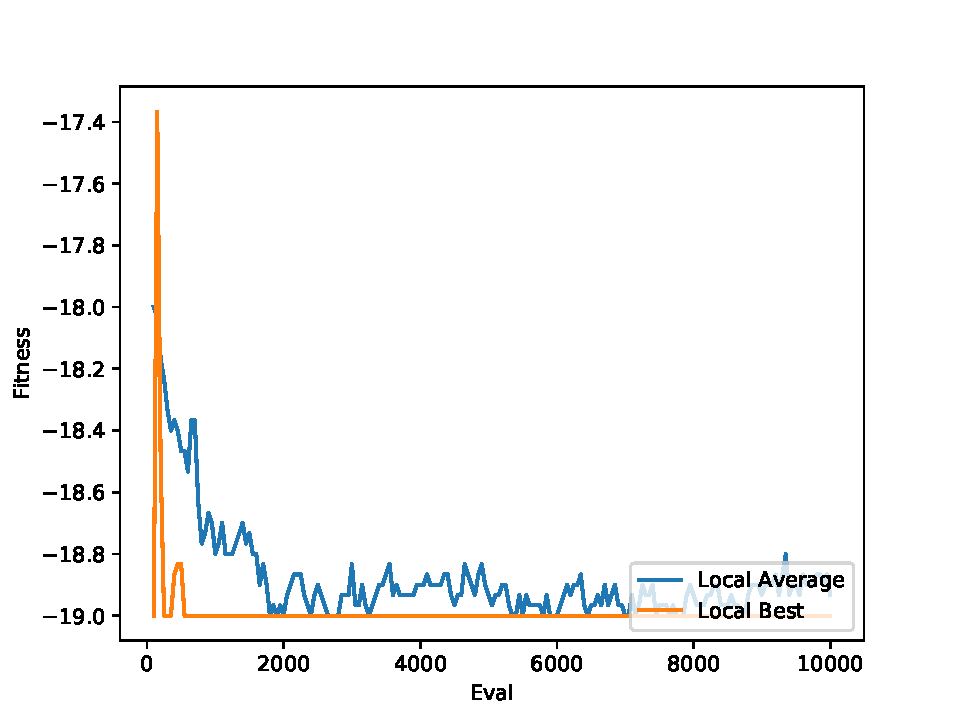
\includegraphics[width=\textwidth]{../graphs/graphs/1007.pdf}
\end{figure}


\begin{figure}[!htb]
	\caption{Figure \ref{fig:graph_1007} Representation}
	\label{fig:picture_1007}
	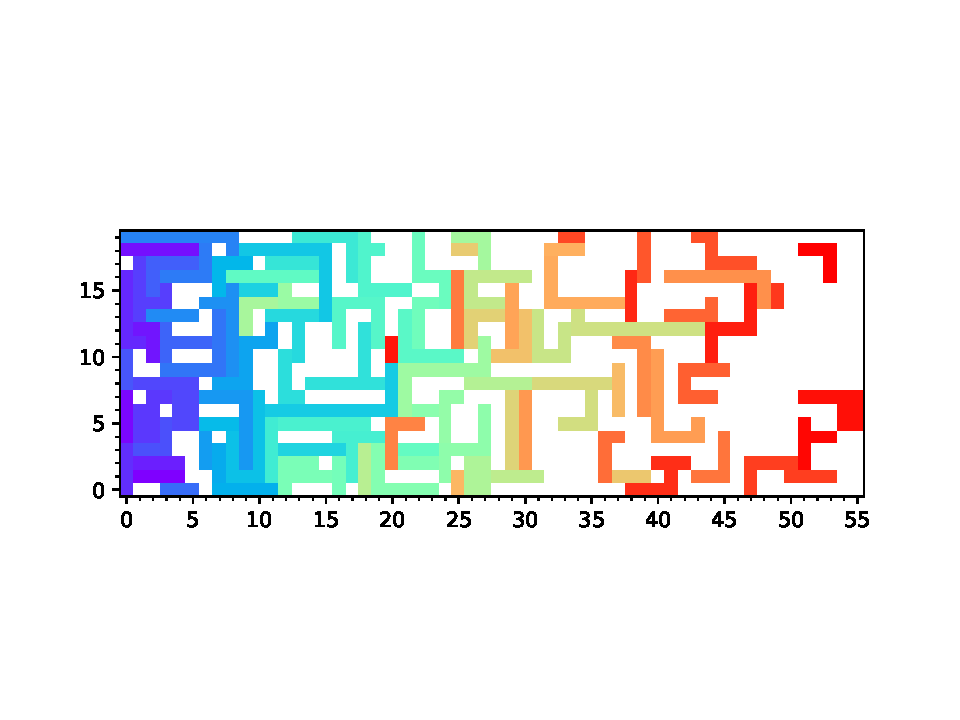
\includegraphics[width=\textwidth]{../graphs/picture/1007.pdf}
\end{figure}


\begin{table}[!htb]
	\centering
	\caption{Figure \ref{fig:graph_1008} Configuration File}
	\label{tab:graph_1008}
	\begin{tabular}{| c | c |}
		\hline
		Mutation Algorithm		& Flip		 \\
		\hline
		Fitness Evaluations		& 10000		 \\
		\hline
		Tournament Size For Survival Selection		& 5		 \\
		\hline
		Mutation Rate		& 0.1		 \\
		\hline
		Self Adaptive Penalty Coefficient		& False		 \\
		\hline
		Random Seed		& 1008		 \\
		\hline
		Population Size		& 100		 \\
		\hline
		Placement Algorithm		& Random		 \\
		\hline
		Termination Convergence Criterion		& 10000		 \\
		\hline
		Survival Strategy		& Plus		 \\
		\hline
		Runs		& 30		 \\
		\hline
		Survivor Algorithm		& Truncation		 \\
		\hline
		Offspring Count		& 50		 \\
		\hline
		Solution File Path		& None		 \\
		\hline
		Self Adaptive Mutation Rate		& False		 \\
		\hline
		Search Algorithm		& EA		 \\
		\hline
		Parent Selection Algorithm		& k-Tournament Selection with replacement		 \\
		\hline
		Self Adaptive Offspring Count		& False		 \\
		\hline
		Log File Path		& None		 \\
		\hline
		MOEA		& True		 \\
		\hline
		Recombination Algorithm		& Partially Mapped Crossover		 \\
		\hline
		Tournament Size For Parent Selection		& 5		 \\
		\hline
		Penalty Coefficient		& 1		 \\
		\hline
	\end{tabular}
\end{table}
\begin{figure}[!htb]
	\caption{Input 1}
	\label{fig:graph_1008}
	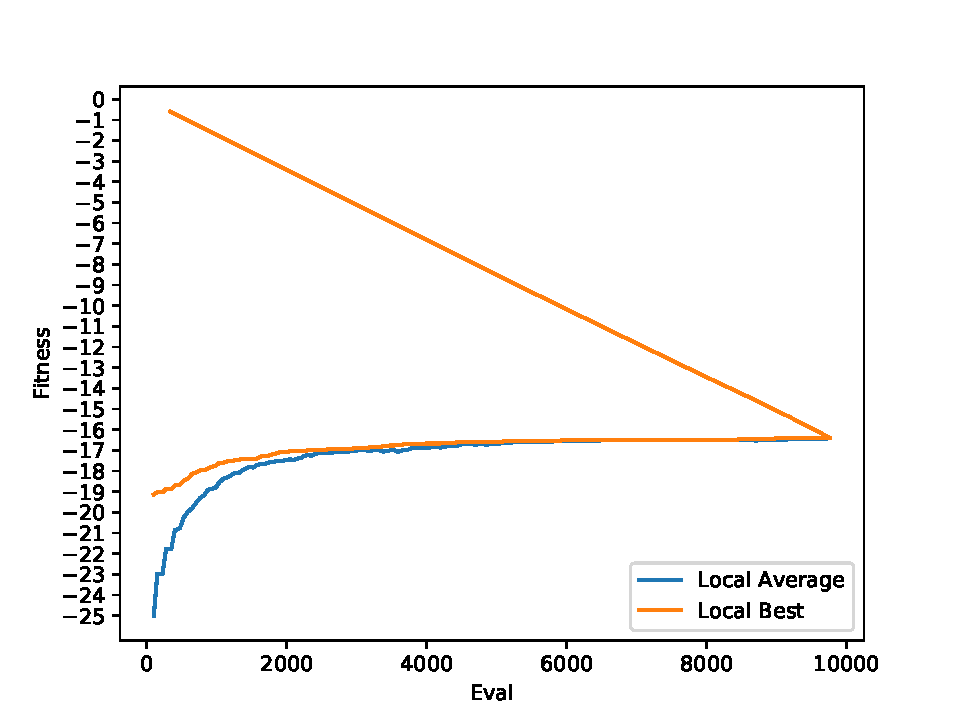
\includegraphics[width=\textwidth]{../graphs/graphs/1008.pdf}
\end{figure}


\begin{figure}[!htb]
	\caption{Figure \ref{fig:graph_1008} Representation}
	\label{fig:picture_1008}
	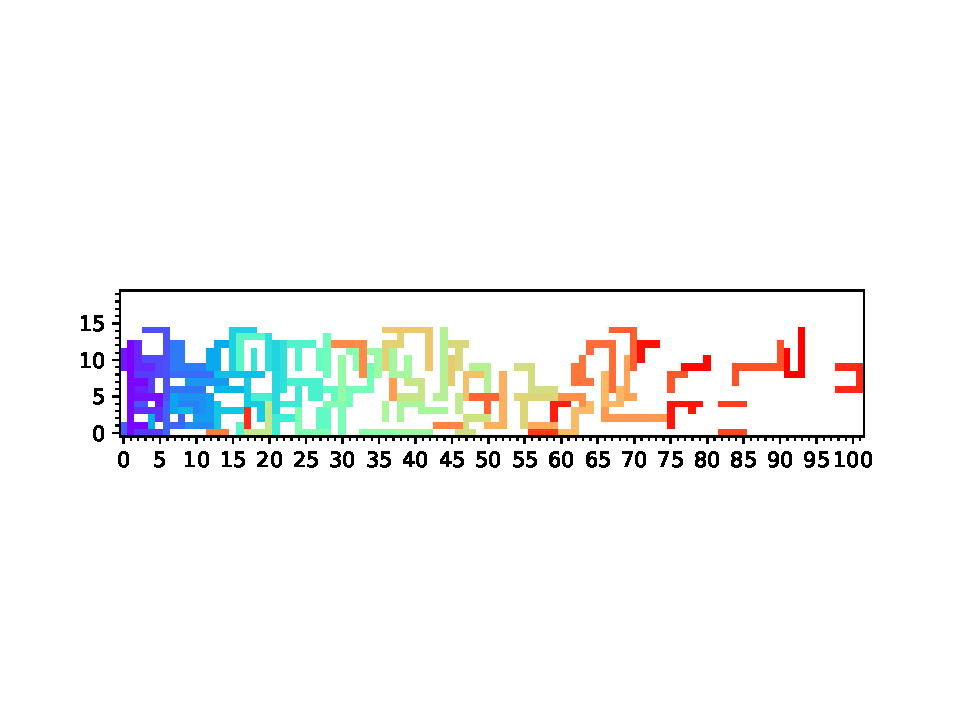
\includegraphics[width=\textwidth]{../graphs/picture/1008.pdf}
\end{figure}


\begin{table}[!htb]
	\centering
	\caption{Figure \ref{fig:graph_1009} Configuration File}
	\label{tab:graph_1009}
	\begin{tabular}{| c | c |}
		\hline
		Mutation Algorithm		& Move		 \\
		\hline
		Fitness Evaluations		& 10000		 \\
		\hline
		Tournament Size For Survival Selection		& 5		 \\
		\hline
		Mutation Rate		& 0.1		 \\
		\hline
		Self Adaptive Penalty Coefficient		& False		 \\
		\hline
		Random Seed		& 1009		 \\
		\hline
		Population Size		& 100		 \\
		\hline
		Placement Algorithm		& Random		 \\
		\hline
		Termination Convergence Criterion		& 10000		 \\
		\hline
		Survival Strategy		& Plus		 \\
		\hline
		Runs		& 30		 \\
		\hline
		Survivor Algorithm		& Truncation		 \\
		\hline
		Offspring Count		& 50		 \\
		\hline
		Solution File Path		& None		 \\
		\hline
		Self Adaptive Mutation Rate		& False		 \\
		\hline
		Search Algorithm		& EA		 \\
		\hline
		Parent Selection Algorithm		& Fitness Proportional Selection		 \\
		\hline
		Self Adaptive Offspring Count		& False		 \\
		\hline
		Log File Path		& None		 \\
		\hline
		MOEA		& True		 \\
		\hline
		Recombination Algorithm		& Partially Mapped Crossover		 \\
		\hline
		Tournament Size For Parent Selection		& 5		 \\
		\hline
		Penalty Coefficient		& 1		 \\
		\hline
	\end{tabular}
\end{table}
\begin{figure}[!htb]
	\caption{Input 1}
	\label{fig:graph_1009}
	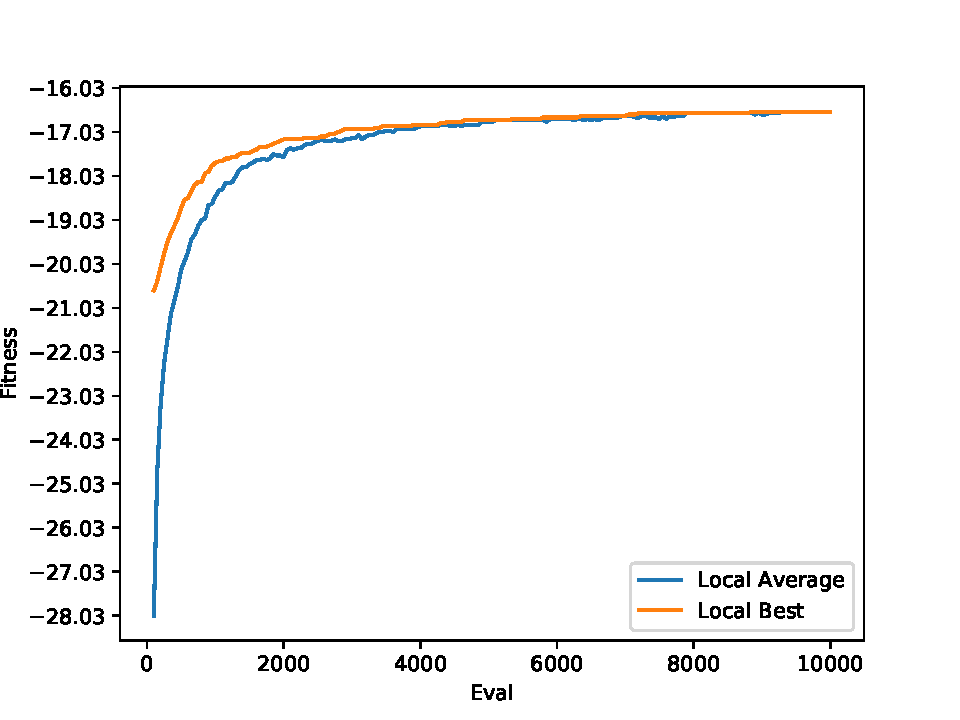
\includegraphics[width=\textwidth]{../graphs/graphs/1009.pdf}
\end{figure}


\begin{figure}[!htb]
	\caption{Figure \ref{fig:graph_1009} Representation}
	\label{fig:picture_1009}
	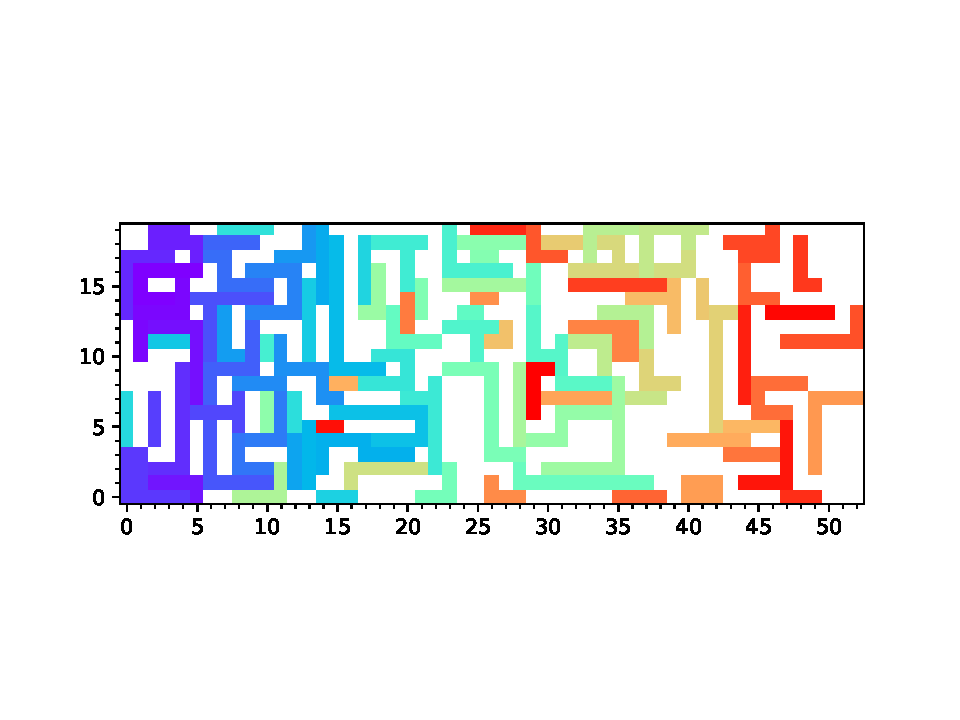
\includegraphics[width=\textwidth]{../graphs/picture/1009.pdf}
\end{figure}


\begin{table}[!htb]
	\centering
	\caption{Figure \ref{fig:graph_1010} Configuration File}
	\label{tab:graph_1010}
	\begin{tabular}{| c | c |}
		\hline
		Mutation Algorithm		& Flip		 \\
		\hline
		Fitness Evaluations		& 10000		 \\
		\hline
		Tournament Size For Survival Selection		& 5		 \\
		\hline
		Mutation Rate		& 0.1		 \\
		\hline
		Self Adaptive Penalty Coefficient		& False		 \\
		\hline
		Random Seed		& 1010		 \\
		\hline
		Population Size		& 100		 \\
		\hline
		Placement Algorithm		& Random		 \\
		\hline
		Termination Convergence Criterion		& 10000		 \\
		\hline
		Survival Strategy		& Plus		 \\
		\hline
		Runs		& 30		 \\
		\hline
		Survivor Algorithm		& Truncation		 \\
		\hline
		Offspring Count		& 50		 \\
		\hline
		Solution File Path		& None		 \\
		\hline
		Self Adaptive Mutation Rate		& False		 \\
		\hline
		Search Algorithm		& EA		 \\
		\hline
		Parent Selection Algorithm		& Fitness Proportional Selection		 \\
		\hline
		Self Adaptive Offspring Count		& False		 \\
		\hline
		Log File Path		& None		 \\
		\hline
		MOEA		& True		 \\
		\hline
		Recombination Algorithm		& Partially Mapped Crossover		 \\
		\hline
		Tournament Size For Parent Selection		& 5		 \\
		\hline
		Penalty Coefficient		& 1		 \\
		\hline
	\end{tabular}
\end{table}
\begin{figure}[!htb]
	\caption{Input 1}
	\label{fig:graph_1010}
	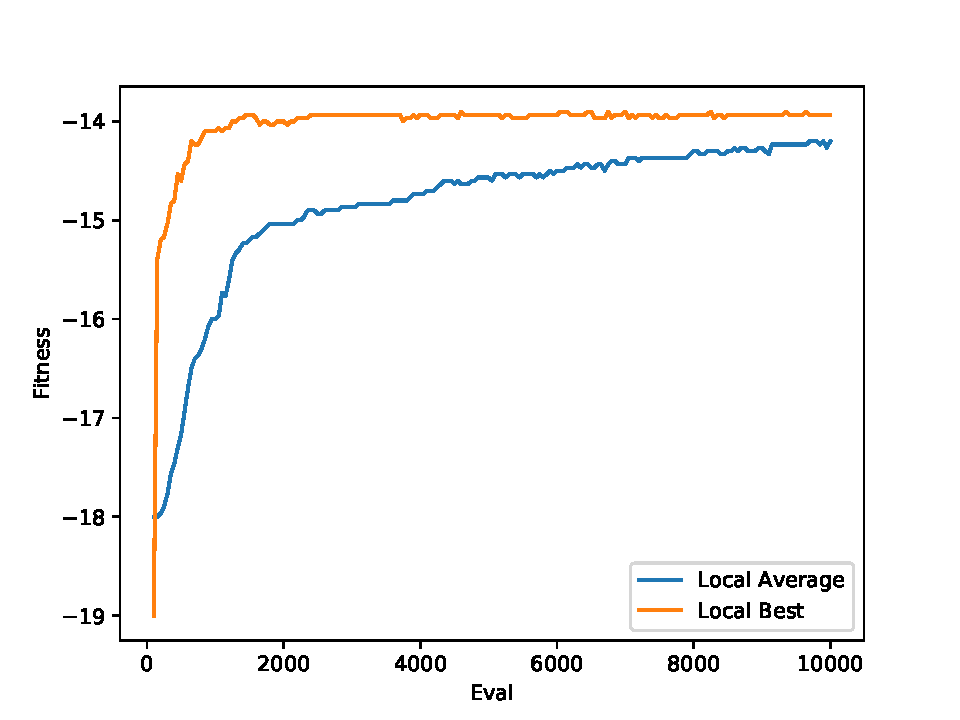
\includegraphics[width=\textwidth]{../graphs/graphs/1010.pdf}
\end{figure}


\begin{figure}[!htb]
	\caption{Figure \ref{fig:graph_1010} Representation}
	\label{fig:picture_1010}
	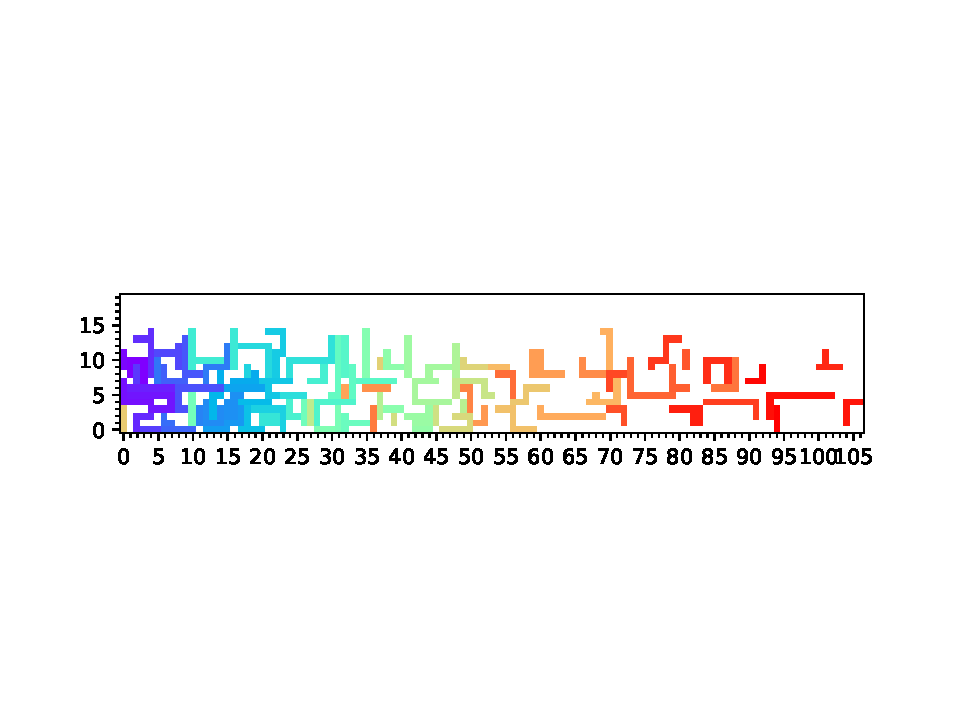
\includegraphics[width=\textwidth]{../graphs/picture/1010.pdf}
\end{figure}


\clearpage
\begin{table}[!htb]
	\centering
	\caption{Figure \ref{fig:graph_1011} Configuration File}
	\label{tab:graph_1011}
	\begin{tabular}{| c | c |}
		\hline
		Mutation Algorithm		& Move		 \\
		\hline
		Fitness Evaluations		& 10000		 \\
		\hline
		Tournament Size For Survival Selection		& 5		 \\
		\hline
		Mutation Rate		& 0.1		 \\
		\hline
		Self Adaptive Penalty Coefficient		& False		 \\
		\hline
		Random Seed		& 1011		 \\
		\hline
		Population Size		& 100		 \\
		\hline
		Placement Algorithm		& Random		 \\
		\hline
		Termination Convergence Criterion		& 10000		 \\
		\hline
		Survival Strategy		& Plus		 \\
		\hline
		Runs		& 30		 \\
		\hline
		Survivor Algorithm		& Truncation		 \\
		\hline
		Offspring Count		& 50		 \\
		\hline
		Solution File Path		& None		 \\
		\hline
		Self Adaptive Mutation Rate		& False		 \\
		\hline
		Search Algorithm		& EA		 \\
		\hline
		Parent Selection Algorithm		& Uniform Random		 \\
		\hline
		Self Adaptive Offspring Count		& False		 \\
		\hline
		Log File Path		& None		 \\
		\hline
		MOEA		& True		 \\
		\hline
		Recombination Algorithm		& Partially Mapped Crossover		 \\
		\hline
		Tournament Size For Parent Selection		& 5		 \\
		\hline
		Penalty Coefficient		& 1		 \\
		\hline
	\end{tabular}
\end{table}
\begin{figure}[!htb]
	\caption{Input 1}
	\label{fig:graph_1011}
	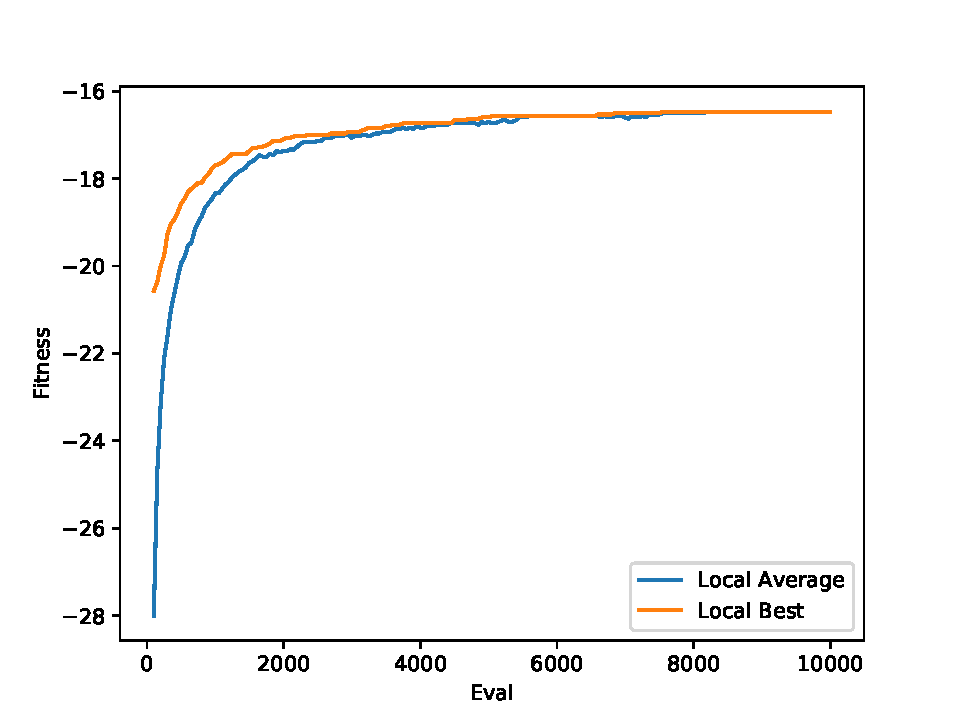
\includegraphics[width=\textwidth]{../graphs/graphs/1011.pdf}
\end{figure}


\begin{figure}[!htb]
	\caption{Figure \ref{fig:graph_1011} Representation}
	\label{fig:picture_1011}
	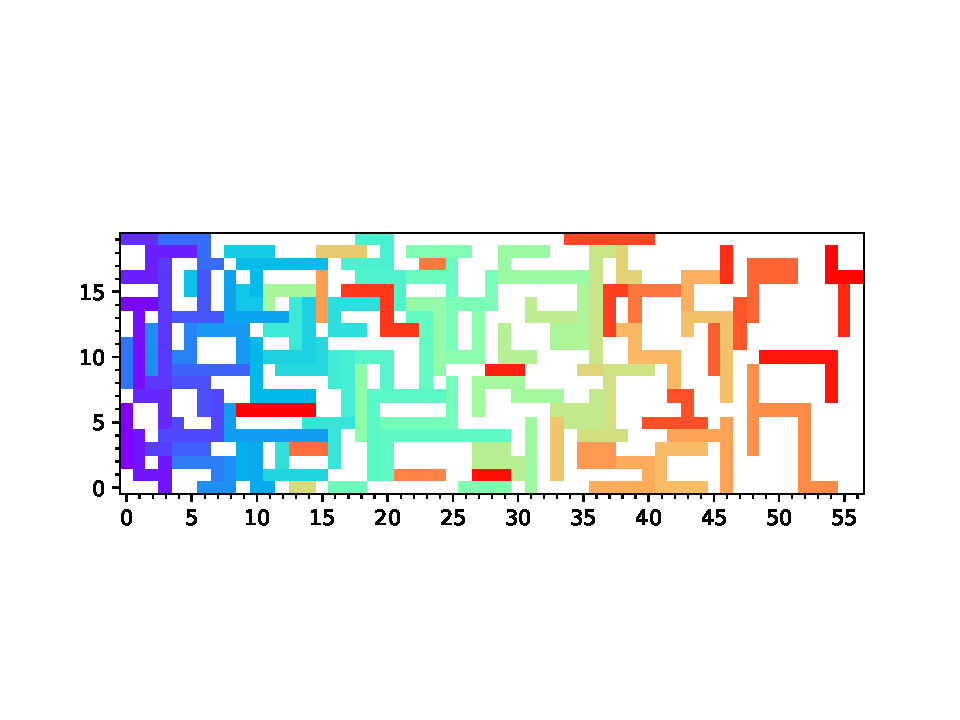
\includegraphics[width=\textwidth]{../graphs/picture/1011.pdf}
\end{figure}


\begin{table}[!htb]
	\centering
	\caption{Figure \ref{fig:graph_1012} Configuration File}
	\label{tab:graph_1012}
	\begin{tabular}{| c | c |}
		\hline
		Mutation Algorithm		& Flip		 \\
		\hline
		Fitness Evaluations		& 10000		 \\
		\hline
		Tournament Size For Survival Selection		& 5		 \\
		\hline
		Mutation Rate		& 0.1		 \\
		\hline
		Self Adaptive Penalty Coefficient		& False		 \\
		\hline
		Random Seed		& 1012		 \\
		\hline
		Population Size		& 100		 \\
		\hline
		Placement Algorithm		& Random		 \\
		\hline
		Termination Convergence Criterion		& 10000		 \\
		\hline
		Survival Strategy		& Plus		 \\
		\hline
		Runs		& 30		 \\
		\hline
		Survivor Algorithm		& Truncation		 \\
		\hline
		Offspring Count		& 50		 \\
		\hline
		Solution File Path		& None		 \\
		\hline
		Self Adaptive Mutation Rate		& False		 \\
		\hline
		Search Algorithm		& EA		 \\
		\hline
		Parent Selection Algorithm		& Uniform Random		 \\
		\hline
		Self Adaptive Offspring Count		& False		 \\
		\hline
		Log File Path		& None		 \\
		\hline
		MOEA		& True		 \\
		\hline
		Recombination Algorithm		& Partially Mapped Crossover		 \\
		\hline
		Tournament Size For Parent Selection		& 5		 \\
		\hline
		Penalty Coefficient		& 1		 \\
		\hline
	\end{tabular}
\end{table}
\begin{figure}[!htb]
	\caption{Input 1}
	\label{fig:graph_1012}
	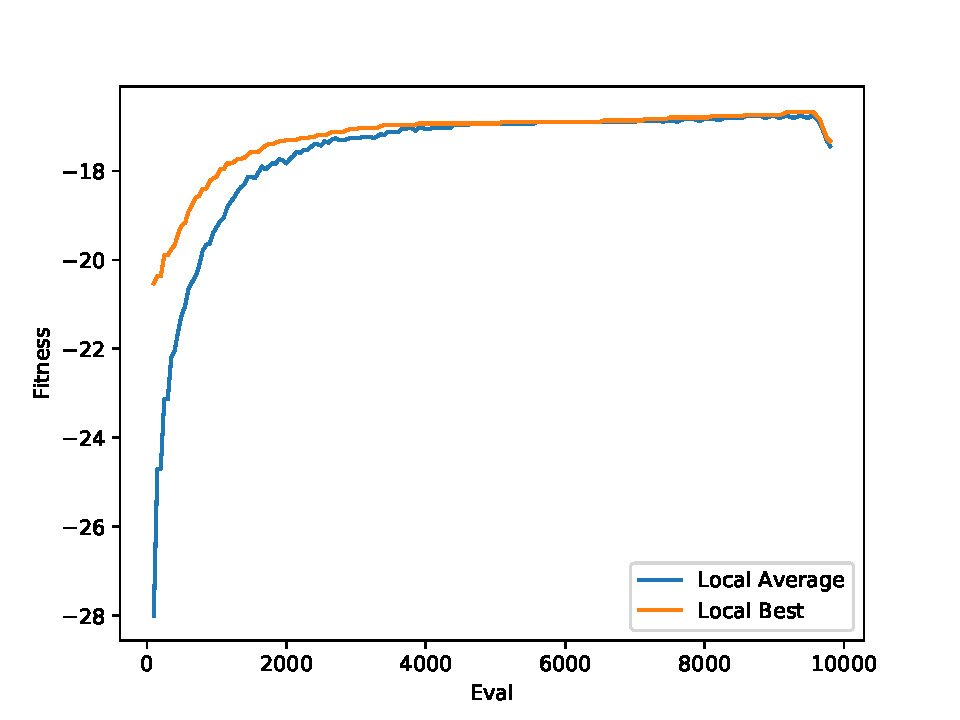
\includegraphics[width=\textwidth]{../graphs/graphs/1012.pdf}
\end{figure}


\begin{figure}[!htb]
	\caption{Figure \ref{fig:graph_1012} Representation}
	\label{fig:picture_1012}
	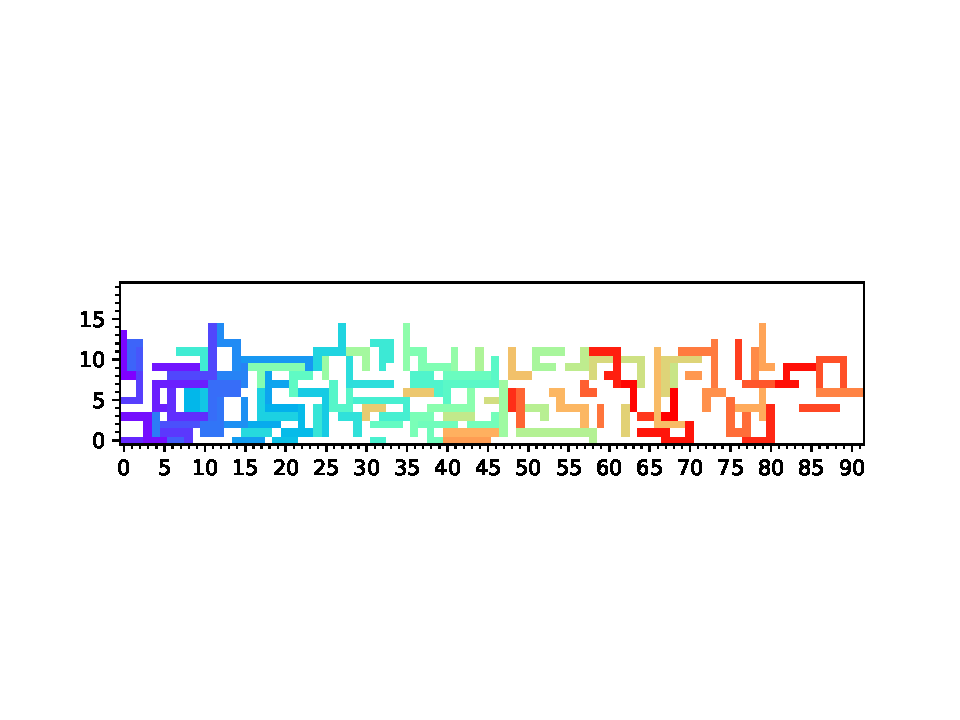
\includegraphics[width=\textwidth]{../graphs/picture/1012.pdf}
\end{figure}


\begin{table}[!htb]
	\centering
	\caption{Figure \ref{fig:graph_1013} Configuration File}
	\label{tab:graph_1013}
	\begin{tabular}{| c | c |}
		\hline
		Mutation Algorithm		& Move		 \\
		\hline
		Fitness Evaluations		& 10000		 \\
		\hline
		Tournament Size For Survival Selection		& 5		 \\
		\hline
		Mutation Rate		& 0.1		 \\
		\hline
		Self Adaptive Penalty Coefficient		& False		 \\
		\hline
		Random Seed		& 1013		 \\
		\hline
		Population Size		& 100		 \\
		\hline
		Placement Algorithm		& Random		 \\
		\hline
		Termination Convergence Criterion		& 10000		 \\
		\hline
		Survival Strategy		& Plus		 \\
		\hline
		Runs		& 30		 \\
		\hline
		Survivor Algorithm		& Truncation		 \\
		\hline
		Offspring Count		& 50		 \\
		\hline
		Solution File Path		& None		 \\
		\hline
		Self Adaptive Mutation Rate		& False		 \\
		\hline
		Search Algorithm		& EA		 \\
		\hline
		Parent Selection Algorithm		& k-Tournament Selection with replacement		 \\
		\hline
		Self Adaptive Offspring Count		& False		 \\
		\hline
		Log File Path		& None		 \\
		\hline
		MOEA		& True		 \\
		\hline
		Recombination Algorithm		& Partially Mapped Crossover		 \\
		\hline
		Tournament Size For Parent Selection		& 5		 \\
		\hline
		Penalty Coefficient		& 1		 \\
		\hline
	\end{tabular}
\end{table}
\begin{figure}[!htb]
	\caption{Input 1}
	\label{fig:graph_1013}
	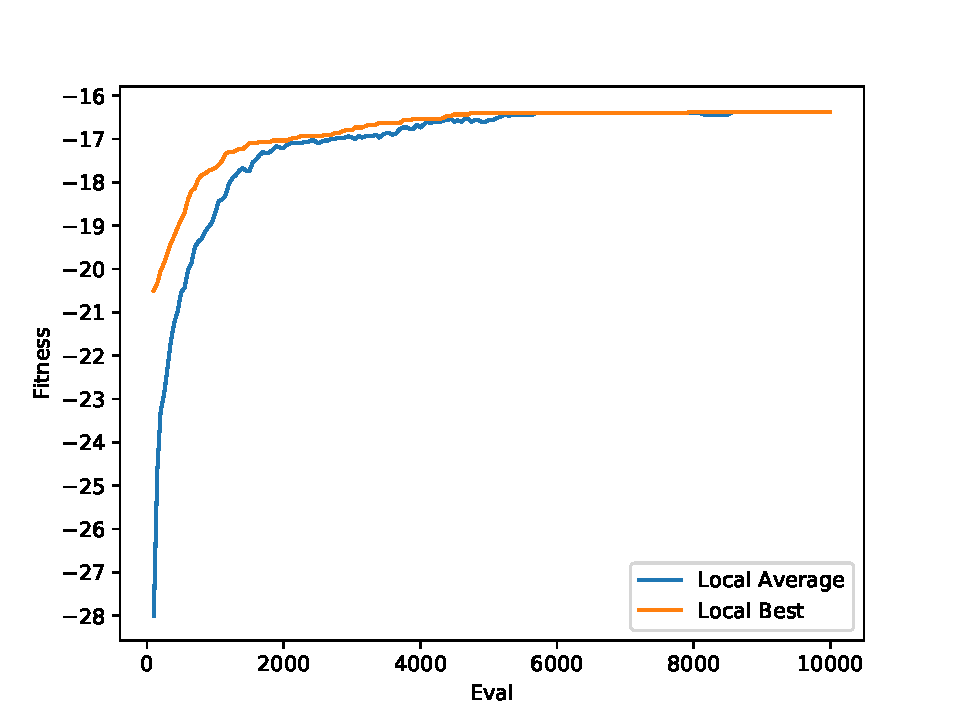
\includegraphics[width=\textwidth]{../graphs/graphs/1013.pdf}
\end{figure}


\begin{figure}[!htb]
	\caption{Figure \ref{fig:graph_1013} Representation}
	\label{fig:picture_1013}
	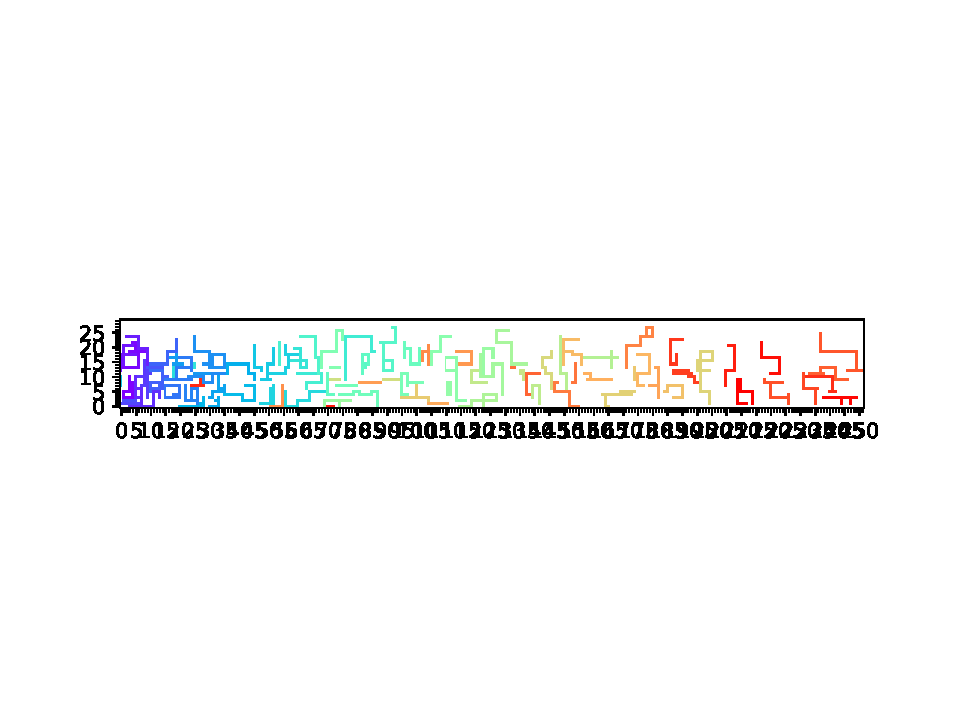
\includegraphics[width=\textwidth]{../graphs/picture/1013.pdf}
\end{figure}


\begin{table}[!htb]
	\centering
	\caption{Figure \ref{fig:graph_1014} Configuration File}
	\label{tab:graph_1014}
	\begin{tabular}{| c | c |}
		\hline
		Mutation Algorithm		& Flip		 \\
		\hline
		Fitness Evaluations		& 10000		 \\
		\hline
		Tournament Size For Survival Selection		& 5		 \\
		\hline
		Mutation Rate		& 0.1		 \\
		\hline
		Self Adaptive Penalty Coefficient		& False		 \\
		\hline
		Random Seed		& 1014		 \\
		\hline
		Population Size		& 100		 \\
		\hline
		Placement Algorithm		& Random		 \\
		\hline
		Termination Convergence Criterion		& 10000		 \\
		\hline
		Survival Strategy		& Plus		 \\
		\hline
		Runs		& 30		 \\
		\hline
		Survivor Algorithm		& Truncation		 \\
		\hline
		Offspring Count		& 50		 \\
		\hline
		Solution File Path		& None		 \\
		\hline
		Self Adaptive Mutation Rate		& False		 \\
		\hline
		Search Algorithm		& EA		 \\
		\hline
		Parent Selection Algorithm		& k-Tournament Selection with replacement		 \\
		\hline
		Self Adaptive Offspring Count		& False		 \\
		\hline
		Log File Path		& None		 \\
		\hline
		MOEA		& True		 \\
		\hline
		Recombination Algorithm		& Partially Mapped Crossover		 \\
		\hline
		Tournament Size For Parent Selection		& 5		 \\
		\hline
		Penalty Coefficient		& 1		 \\
		\hline
	\end{tabular}
\end{table}
\begin{figure}[!htb]
	\caption{Input 1}
	\label{fig:graph_1014}
	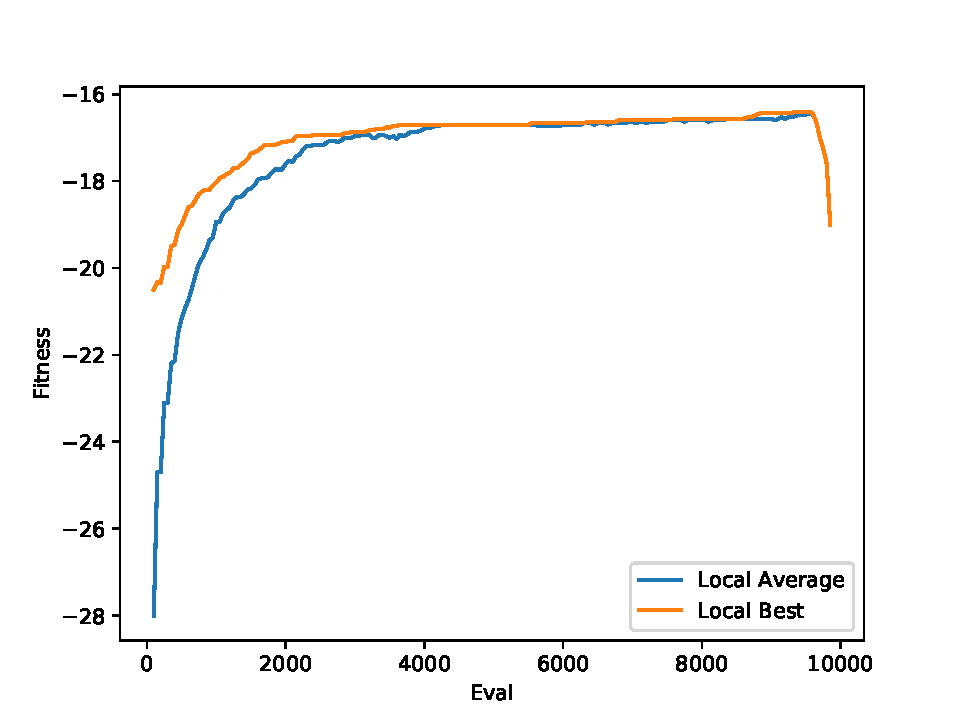
\includegraphics[width=\textwidth]{../graphs/graphs/1014.pdf}
\end{figure}


\begin{figure}[!htb]
	\caption{Figure \ref{fig:graph_1014} Representation}
	\label{fig:picture_1014}
	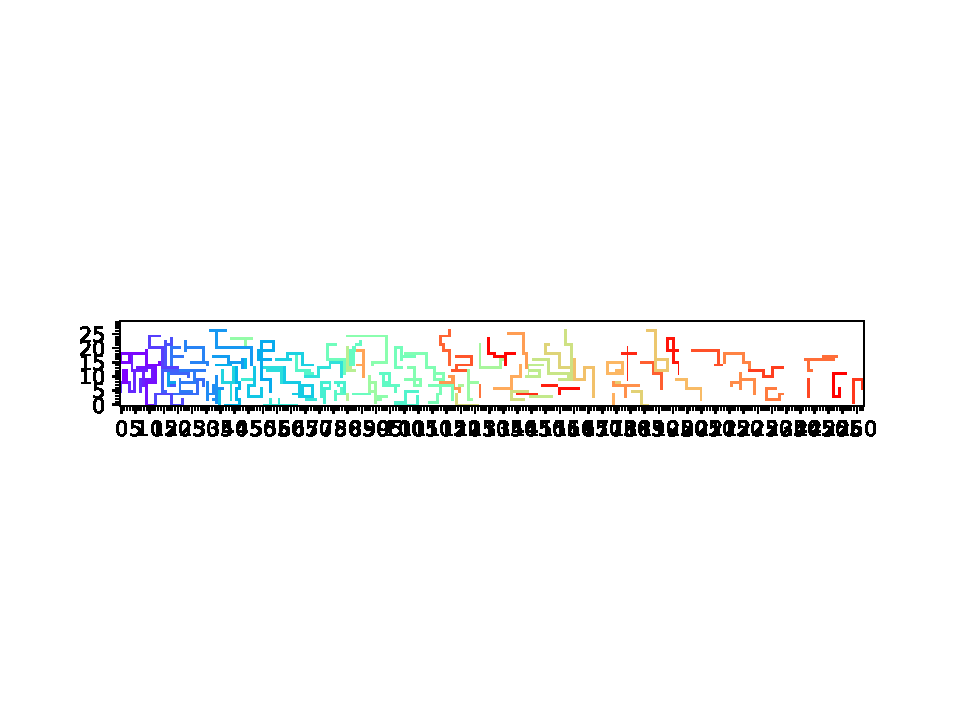
\includegraphics[width=\textwidth]{../graphs/picture/1014.pdf}
\end{figure}


\begin{table}[!htb]
	\centering
	\caption{Figure \ref{fig:graph_1015} Configuration File}
	\label{tab:graph_1015}
	\begin{tabular}{| c | c |}
		\hline
		Mutation Algorithm		& Move		 \\
		\hline
		Fitness Evaluations		& 10000		 \\
		\hline
		Tournament Size For Survival Selection		& 5		 \\
		\hline
		Mutation Rate		& 0.1		 \\
		\hline
		Self Adaptive Penalty Coefficient		& False		 \\
		\hline
		Random Seed		& 1015		 \\
		\hline
		Population Size		& 100		 \\
		\hline
		Placement Algorithm		& Random		 \\
		\hline
		Termination Convergence Criterion		& 10000		 \\
		\hline
		Survival Strategy		& Plus		 \\
		\hline
		Runs		& 30		 \\
		\hline
		Survivor Algorithm		& Truncation		 \\
		\hline
		Offspring Count		& 50		 \\
		\hline
		Solution File Path		& None		 \\
		\hline
		Self Adaptive Mutation Rate		& False		 \\
		\hline
		Search Algorithm		& EA		 \\
		\hline
		Parent Selection Algorithm		& Fitness Proportional Selection		 \\
		\hline
		Self Adaptive Offspring Count		& False		 \\
		\hline
		Log File Path		& None		 \\
		\hline
		MOEA		& True		 \\
		\hline
		Recombination Algorithm		& Partially Mapped Crossover		 \\
		\hline
		Tournament Size For Parent Selection		& 5		 \\
		\hline
		Penalty Coefficient		& 1		 \\
		\hline
	\end{tabular}
\end{table}
\begin{figure}[!htb]
	\caption{Input 1}
	\label{fig:graph_1015}
	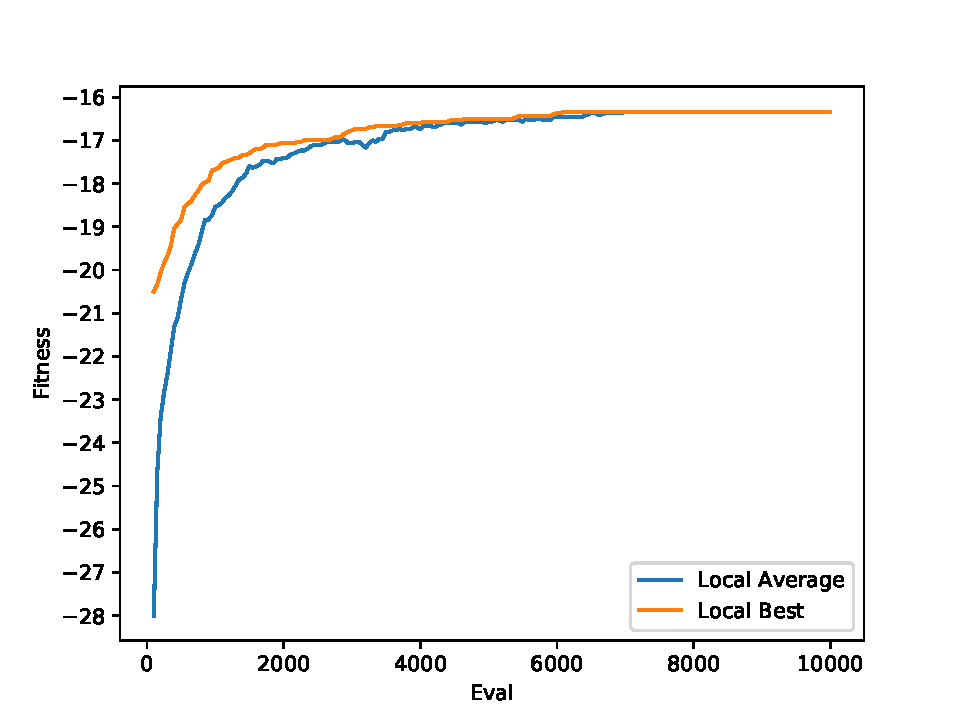
\includegraphics[width=\textwidth]{../graphs/graphs/1015.pdf}
\end{figure}


\begin{figure}[!htb]
	\caption{Figure \ref{fig:graph_1015} Representation}
	\label{fig:picture_1015}
	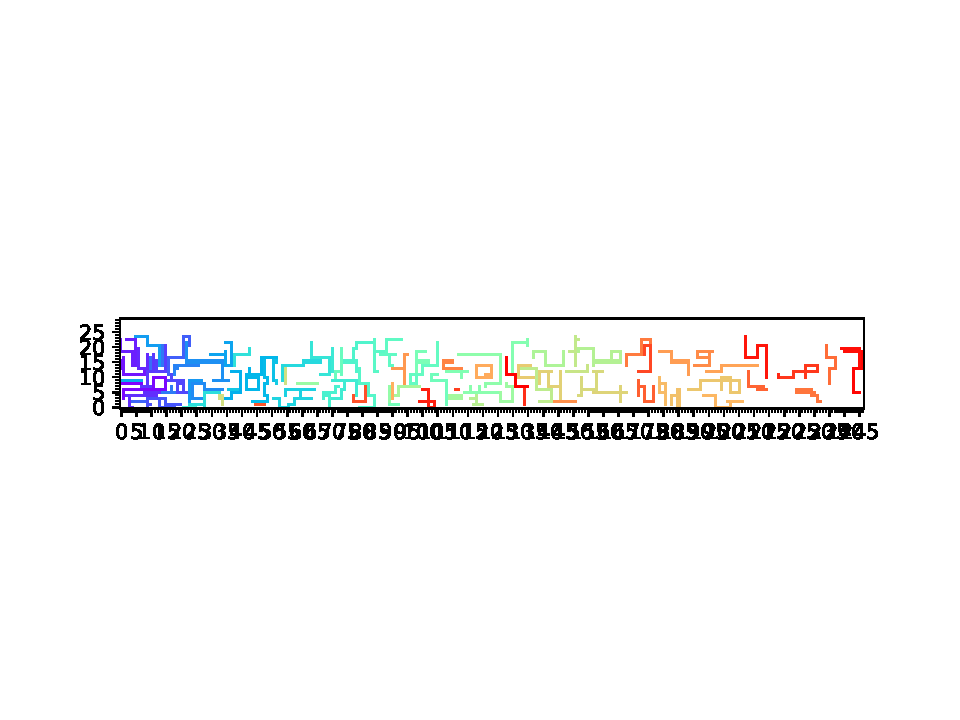
\includegraphics[width=\textwidth]{../graphs/picture/1015.pdf}
\end{figure}


\begin{table}[!htb]
	\centering
	\caption{Figure \ref{fig:graph_1016} Configuration File}
	\label{tab:graph_1016}
	\begin{tabular}{| c | c |}
		\hline
		Mutation Algorithm		& Flip		 \\
		\hline
		Fitness Evaluations		& 10000		 \\
		\hline
		Tournament Size For Survival Selection		& 5		 \\
		\hline
		Mutation Rate		& 0.1		 \\
		\hline
		Self Adaptive Penalty Coefficient		& False		 \\
		\hline
		Random Seed		& 1016		 \\
		\hline
		Population Size		& 100		 \\
		\hline
		Placement Algorithm		& Random		 \\
		\hline
		Termination Convergence Criterion		& 10000		 \\
		\hline
		Survival Strategy		& Plus		 \\
		\hline
		Runs		& 30		 \\
		\hline
		Survivor Algorithm		& Truncation		 \\
		\hline
		Offspring Count		& 50		 \\
		\hline
		Solution File Path		& None		 \\
		\hline
		Self Adaptive Mutation Rate		& False		 \\
		\hline
		Search Algorithm		& EA		 \\
		\hline
		Parent Selection Algorithm		& Fitness Proportional Selection		 \\
		\hline
		Self Adaptive Offspring Count		& False		 \\
		\hline
		Log File Path		& None		 \\
		\hline
		MOEA		& True		 \\
		\hline
		Recombination Algorithm		& Partially Mapped Crossover		 \\
		\hline
		Tournament Size For Parent Selection		& 5		 \\
		\hline
		Penalty Coefficient		& 1		 \\
		\hline
	\end{tabular}
\end{table}
\begin{figure}[!htb]
	\caption{Input 1}
	\label{fig:graph_1016}
	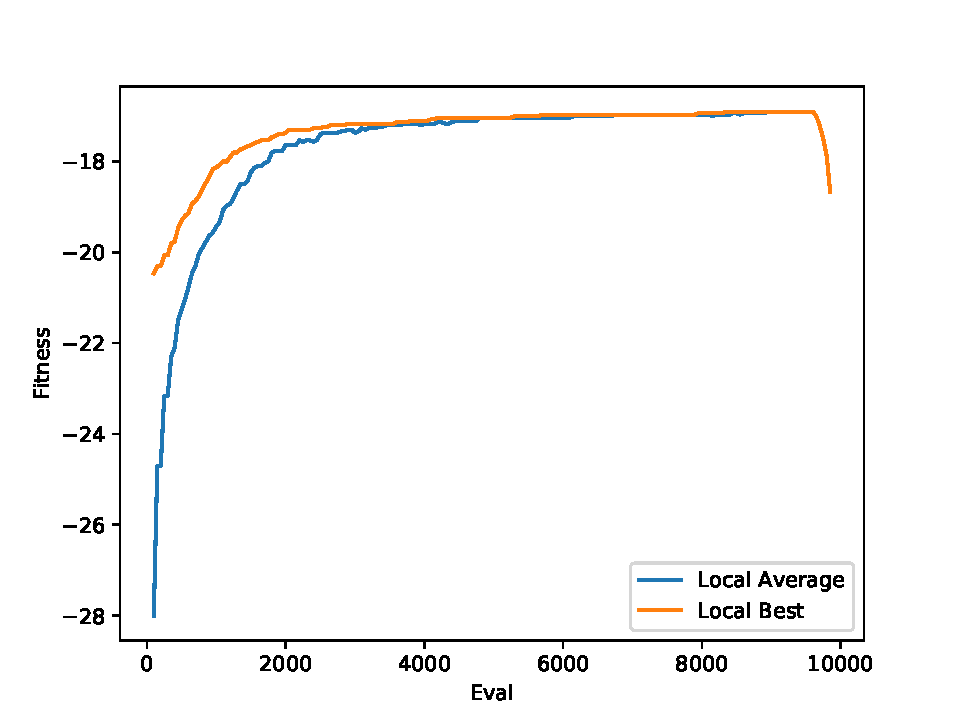
\includegraphics[width=\textwidth]{../graphs/graphs/1016.pdf}
\end{figure}


\begin{figure}[!htb]
	\caption{Figure \ref{fig:graph_1016} Representation}
	\label{fig:picture_1016}
	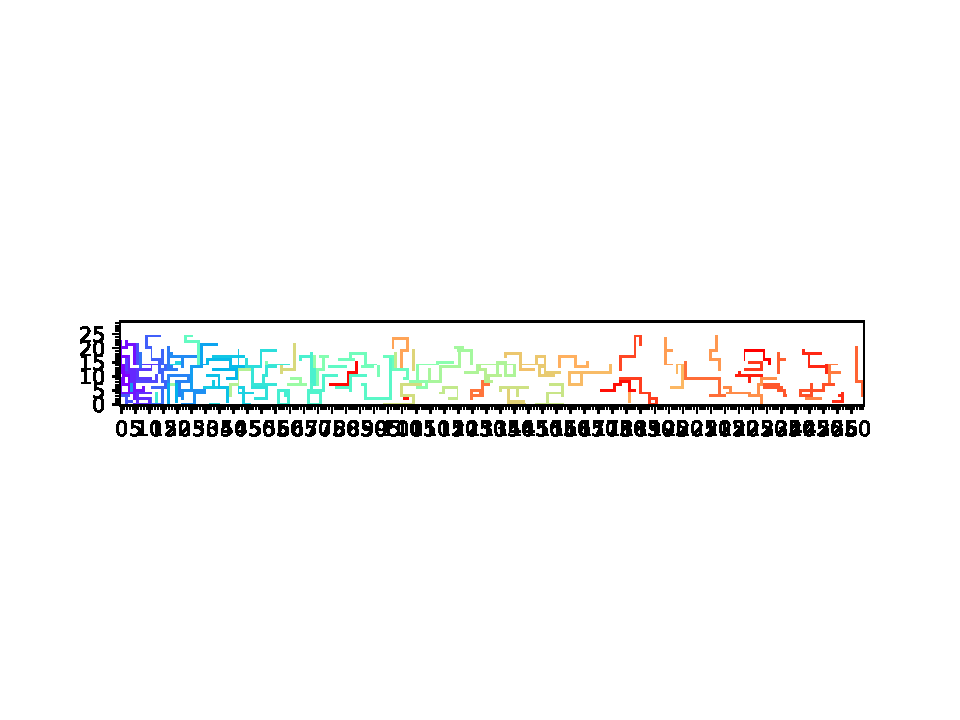
\includegraphics[width=\textwidth]{../graphs/picture/1016.pdf}
\end{figure}


\begin{table}[!htb]
	\centering
	\caption{Figure \ref{fig:graph_1017} Configuration File}
	\label{tab:graph_1017}
	\begin{tabular}{| c | c |}
		\hline
		Mutation Algorithm		& Move		 \\
		\hline
		Fitness Evaluations		& 10000		 \\
		\hline
		Tournament Size For Survival Selection		& 5		 \\
		\hline
		Mutation Rate		& 0.1		 \\
		\hline
		Self Adaptive Penalty Coefficient		& False		 \\
		\hline
		Random Seed		& 1017		 \\
		\hline
		Population Size		& 100		 \\
		\hline
		Placement Algorithm		& Random		 \\
		\hline
		Termination Convergence Criterion		& 10000		 \\
		\hline
		Survival Strategy		& Plus		 \\
		\hline
		Runs		& 30		 \\
		\hline
		Survivor Algorithm		& Truncation		 \\
		\hline
		Offspring Count		& 50		 \\
		\hline
		Solution File Path		& None		 \\
		\hline
		Self Adaptive Mutation Rate		& False		 \\
		\hline
		Search Algorithm		& EA		 \\
		\hline
		Parent Selection Algorithm		& Uniform Random		 \\
		\hline
		Self Adaptive Offspring Count		& False		 \\
		\hline
		Log File Path		& None		 \\
		\hline
		MOEA		& True		 \\
		\hline
		Recombination Algorithm		& Partially Mapped Crossover		 \\
		\hline
		Tournament Size For Parent Selection		& 5		 \\
		\hline
		Penalty Coefficient		& 1		 \\
		\hline
	\end{tabular}
\end{table}
\begin{figure}[!htb]
	\caption{Input 1}
	\label{fig:graph_1017}
	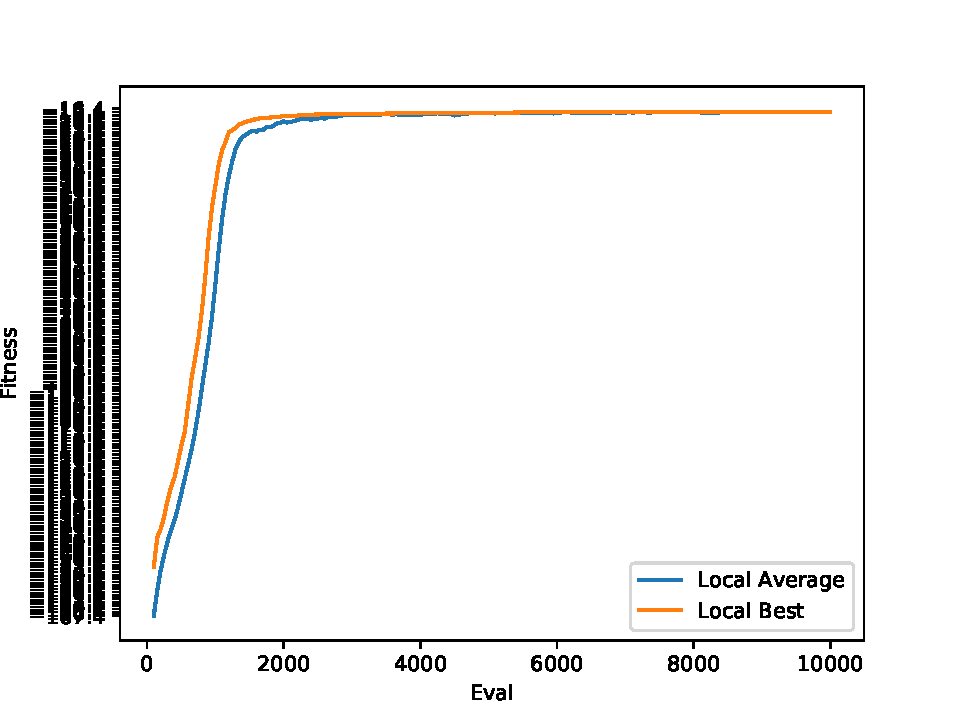
\includegraphics[width=\textwidth]{../graphs/graphs/1017.pdf}
\end{figure}


\begin{figure}[!htb]
	\caption{Figure \ref{fig:graph_1017} Representation}
	\label{fig:picture_1017}
	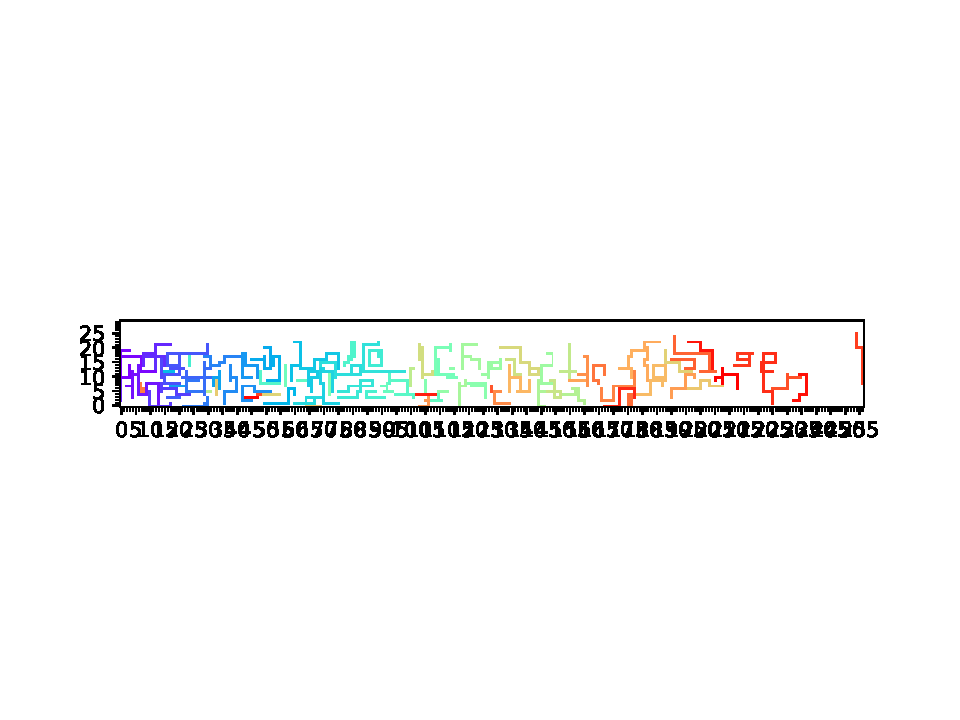
\includegraphics[width=\textwidth]{../graphs/picture/1017.pdf}
\end{figure}


\begin{table}[!htb]
	\centering
	\caption{Figure \ref{fig:graph_1018} Configuration File}
	\label{tab:graph_1018}
	\begin{tabular}{| c | c |}
		\hline
		Mutation Algorithm		& Flip		 \\
		\hline
		Fitness Evaluations		& 10000		 \\
		\hline
		Tournament Size For Survival Selection		& 5		 \\
		\hline
		Mutation Rate		& 0.1		 \\
		\hline
		Self Adaptive Penalty Coefficient		& False		 \\
		\hline
		Random Seed		& 1018		 \\
		\hline
		Population Size		& 100		 \\
		\hline
		Placement Algorithm		& Random		 \\
		\hline
		Termination Convergence Criterion		& 10000		 \\
		\hline
		Survival Strategy		& Plus		 \\
		\hline
		Runs		& 30		 \\
		\hline
		Survivor Algorithm		& Truncation		 \\
		\hline
		Offspring Count		& 50		 \\
		\hline
		Solution File Path		& None		 \\
		\hline
		Self Adaptive Mutation Rate		& False		 \\
		\hline
		Search Algorithm		& EA		 \\
		\hline
		Parent Selection Algorithm		& Uniform Random		 \\
		\hline
		Self Adaptive Offspring Count		& False		 \\
		\hline
		Log File Path		& None		 \\
		\hline
		MOEA		& True		 \\
		\hline
		Recombination Algorithm		& Partially Mapped Crossover		 \\
		\hline
		Tournament Size For Parent Selection		& 5		 \\
		\hline
		Penalty Coefficient		& 1		 \\
		\hline
	\end{tabular}
\end{table}
\begin{figure}[!htb]
	\caption{Input 1}
	\label{fig:graph_1018}
	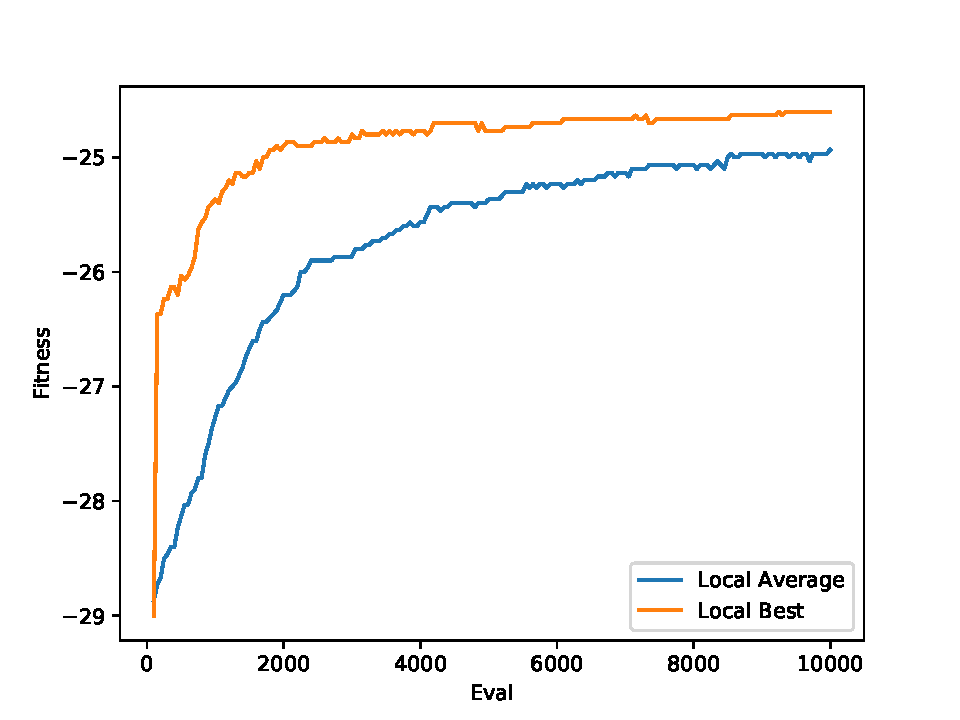
\includegraphics[width=\textwidth]{../graphs/graphs/1018.pdf}
\end{figure}


\begin{figure}[!htb]
	\caption{Figure \ref{fig:graph_1018} Representation}
	\label{fig:picture_1018}
	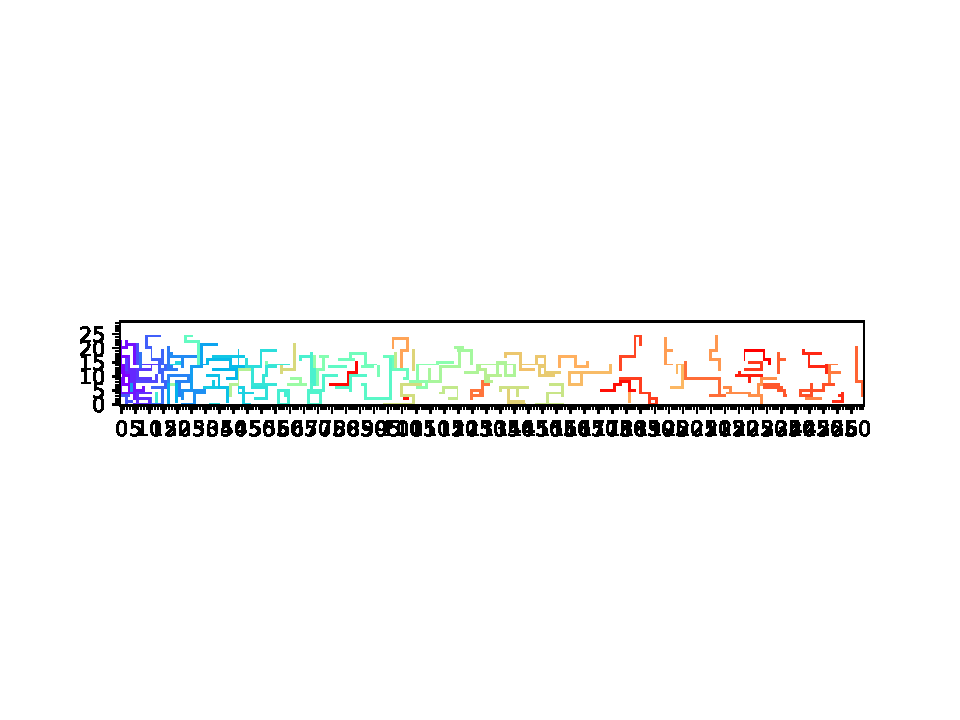
\includegraphics[width=\textwidth]{../graphs/picture/1018.pdf}
\end{figure}


\end{document}
